\chapter{向量与向量运算}
在常用的数量问题中,我们用数去表达各种量,如重
量、长度、面积、体积、密度等等;用加、减、乘、除运算
的组合去表达各种量之间的关系(通称代数通性).在代数
中,我们已掌握了数系的基本性质(即交换律、结合律和分
配律).并熟知了代数学的基本精神在于有效地运用数系
通性,对于各种类型的代数问题谋求通解(即以通性求通
解).现在我们要着手把几何学的讨论也推进到定量的层
面,设法把空间结构有系统地代数化,数量化,这也就是本
章所要详加讨论的课题——\textbf{向量与向量运算}.为了便于同学
们逐步地理解向量这个基本概念,本章的前三节先对平面向
量详加分析,然后再在第四节讨论空间向量.

\section{平面位移向量及其加法运算}

\subsection{位移向量}

如图3.1所示,我们在$\overline{AB}$的端点$B$处画	
上一个箭头表示 线段$\overline{AB}$具有射线$AB$的方向,这种用箭头指明方向的线段叫做\textbf{有向线段},记作$\Vec{AB}$,读作有向线段$AB$,并称A为$\Vec{AB}$的\textbf{始点},$B$为$\Vec{AB}$的\textbf{终点}.$\overline{AB}$的长叫做$\Vec{AB}$的长,并记作$|\Vec{AB}|$.

$\Vec{AB}$和$\Vec{CD}$同向且等长,那么我们称$\Vec{AB}$和$\Vec{CD}$\textbf{相等},记作$\Vec{AB}=\Vec{CD}$(图3.2).

\begin{figure}[htp]\centering
    \begin{minipage}[t]{0.48\textwidth}
    \centering
\begin{tikzpicture}[>=latex, scale=.8]
    \draw[->](0,0)node[below]{$A$}--(2,3)node[above]{$B$};
    \end{tikzpicture}
    \caption{}
    \end{minipage}
    \begin{minipage}[t]{0.48\textwidth}
    \centering
    \begin{tikzpicture}[>=latex, scale=.8]
        \draw[->](0,0)node[below]{$A$}--(2,3)node[above]{$B$};
        \draw [dashed](0,0)--(3,.5);\draw [dashed](2,3)--(5,3.5);
        \draw[->](3,.5)node[below]{$C$}--(5,3.5)node[above]{$D$};
    \end{tikzpicture}
    \caption{}
    \end{minipage}
    \end{figure}

已知方向$ON$(图3.3), 如果平面上的每一点都沿射线
$ON$的方向移动相同的距离,那
么我们称这种平面上全体点的移
动叫做平面上全体点的一个\textbf{平移}.

\begin{figure}[htp]\centering
    \begin{minipage}[t]{0.48\textwidth}
    \centering
\begin{tikzpicture}[>=latex, xscale=.8]
       \draw[->] (0,0)node[right]{$O$}--(0,1)node[right]{$N$};
       \draw[dashed](0,1)--(0,2.5);
\draw[->] (1,0)node[right]{$P$}--(1,2)node[right]{$P_1$};
\draw[->] (2,1)--(2,3);  \draw[->] (3,.5)--(3,2.5);  
\draw[->] (4,1)--(4,3);  \draw[->] (5,.5)--(5,2.5);  
    \end{tikzpicture}
    \caption{}
    \end{minipage}
    \begin{minipage}[t]{0.48\textwidth}
    \centering
    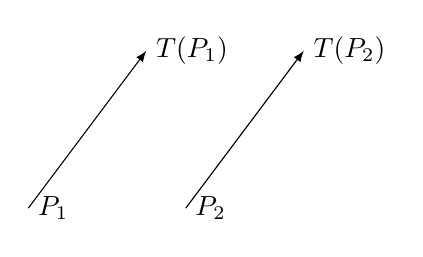
\begin{tikzpicture}[>=latex, scale=1]
        \draw[->] (0,0)node[right]{$P_1$}--(1.5,2)node[right]{$T(P_1)$};
        \draw[->] (2,0)node[right]{$P_2$}--(3.5,2)node[right]{$T(P_2)$};
    \end{tikzpicture}
    \caption{}
    \end{minipage}
    \end{figure}

平面上全体点的一个平移通
常用字母$T$来表示,不同的平移可分别用$T_1,T_2,\ldots$来表示.
如果$P$点通过平移$T$移动到$P_1$点,则$P_1$点叫做$P$点的\textbf{象
点},记作$P_1=T(P)$, 这时有向线段$\Vec{PP_1}$; 可写作$\Vec{PT(P)}$.

为了给出一个平移,根据定义,只需给出平面上任一点
和它的象点即可.设$P_1=T(P)$, 则$P$、$P_1$这两点 就完全
确定了平移$T$的方向和距离;对平面上任一点$A$, 我们都
可作$\Vec{AA_1}=\Vec{PP_1}$, 这样$A$的象点$A_1$也就被$\Vec{PP_1}$所唯一确
定,这也就是说,给定了一个平移$T$, 如果$P_1=T(P)$, 那
么这个平移$T$完全被$\Vec{PT(P)}$所唯一确定,通常我们就用
$\Vec{PT(P)}$或$\Vec{PP_1}$表示这个平移.

显然,平面上全体点的一个移动是一个平移的充要条件
是:对平面上任意两点$P_1$、$P_2$,都有
\[\Vec{P_1T(P_1)}=\Vec{P_2T(P_2)}\]

从以上讨论知,一个平移$T$只有两个要素:\textbf{方向和距离},
因此平面上的一个平移$T$, 可用
那些同向且等长的任一条有向线段来表示.

几次连续平移的结果,叫做平移的\textbf{合成}.设$T_1$、$T_2$是
两次连续平移,这两次连续平移的合成通常记作$T_2\circ T_1$(第
一次平移写在右边),类似地$T_3\circ T_2\circ T_1$, 表示$T_1$、$T_2$、$T_3$三
次连续平移的合成.

\begin{blk}{定理}
    平移的合成还是一个平移且平移的合成满足交换
律.
\end{blk}

\begin{proof}
设$T_1$、$T_2$是两个平移,我们要证明的是:$T_2\circ T_1$也是一个平移,$T_2\circ T_1=T_1\circ T_2$.

设$P$、$Q$是平面上任意两点(图3.5),$P_1=T_1(P)$、
$P_2=T_2(P_1)$、$Q_1=T_1(Q)$、$Q_2=T_2(Q_1)$, 则$P_2=T_2(T_1(P))$, $Q_2=T_2(T_1(Q))$
\begin{figure}[htp]
    \centering
\begin{tikzpicture}[>=latex]
\tkzDefPoints{0/0/P, .85/2/P_1, 2/3/P_2, 4/0/Q}
\tkzDefPointsBy[translation= from P to Q](P_1,P_2){Q_1,Q_2}
\draw[->](P) -- node[left]{$T_1$} (P_1);
\draw[->](Q) -- node[left]{$T_1$} (Q_1);
\draw[->](P) --  (P_2);
\draw[->](Q) -- (Q_2);
\draw[->](P_1) -- node[left]{$T_2$} (P_2);
\draw[->](Q_1) -- node[left]{$T_2$} (Q_2);
\tkzDrawSegments(P,Q P_2,Q_2 P_1,Q_1)
\tkzLabelPoints[left](P_2,Q_2,P_1,Q_1)
\tkzLabelPoints[below](P,Q)
\end{tikzpicture}
    \caption{}
\end{figure}

我们要证明$T_2\circ T_1$是一个平移也就是要证
明$\overline{PP_2}$与$\overline{QQ_2}$平行且等
长.即
\[\Vec{PP_2}=\Vec{QQ_2}\]
由于$T_1$、$T_2$都是平移,则
\[\Vec{PP_1}=\Vec{QQ_1},\qquad \Vec{P_1P_2}=\Vec{Q_1Q_2}\]
连$P$、$P_2$, $Q$、$Q_2$由平行四边形基本定理(即\textbf{一个四边形的
一组对边平行且等长,则另一组对边也平行且等长}),容易
证明:
\[\Vec{PP_2}=\Vec{QQ_2}\]
这就证明了$T_2\circ T_1$也是一个平移.



设点$P$是平面上任一点,$P_1=T_1(P)$, $P_2=T_2(P_1)$,
则$P_2=T_2(T_1(P))$, 这就是说$T_2\circ T_1$把$P$点移动到$P_2$点.

设$Q=T_2(P)$, 由平移定义可知
\[\Vec{P_1P_2}=\Vec{PQ}\]
又由上述平行四边形基本定理可证
\[\Vec{PP_1}=\Vec{QP_2}\]
这就是说
\[P_2=T_1(Q)=T_1(T_2(P))\]
所以
\[T_2\circ T_1=T_1\circ T_2\]
\end{proof}

\begin{figure}[htp]\centering
    \begin{minipage}[t]{0.48\textwidth}
    \centering
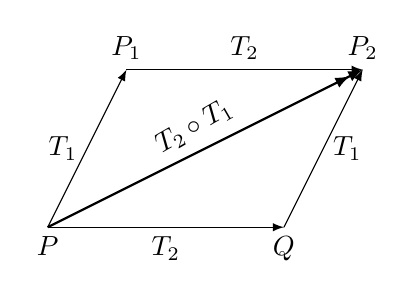
\begin{tikzpicture}[>=latex, scale=1]
    \draw[->](0,0)node[below]{$P$}--node[below]{$T_2$}(3,0) node[below]{$Q$} ;
    \draw[->](0,0)--node[left]{$T_1$}(1,2)node[above]{$P_1$}  ;
    \draw[->](3,0)--node[right]{$T_1$}(4,2)node[above]{$P_2$};
    \draw[->>, thick](0,0)--node[above=1pt, rotate=30]{$T_2\circ T_1$}(4,2)  ;
    \draw[->](1,2)--node[above]{$T_2$}(4,2)  ;
    \end{tikzpicture}
    \caption{}
    \end{minipage}
    \begin{minipage}[t]{0.48\textwidth}
    \centering
    \begin{tikzpicture}[>=latex, scale=.8]
        \draw[->](0,0)--node[below]{$T_1$}(4,0);
        \draw[->](0,0)--node[left]{$T_2$}(0,4);
        \draw[->>](0,0)--node[above, rotate=45]{$5\sqrt{2}$}(4,4);
        \draw[->](4,0)--node[right]{$T_2$}(4,4);
        \draw[->](0,4)--node[above]{$T_1$}(4,4);

        \draw[->](-1,2)--(-1,3)node[left]{北};
    \end{tikzpicture}
    \caption{}
    \end{minipage}
    \end{figure}


\begin{example}
    已知$T_1$表示平移“向东5公里”,$T_2$表示平移
“向北5公里”,求$T_1\circ T_2$, $T_2\circ T_1$.
\end{example}

\begin{solution}
    $T_1\circ T_2=T_2\circ T_1$都表示平移:“向东北$5\sqrt{2}$公里”(图3.7)
\end{solution}

\begin{example}
    已知:$T_1:$ “向东5公里”,$T_2:$ “向西10公里”,求$T_1\circ T_2$和$T_2\circ T_1$.
\end{example}

\begin{solution}
   $T_1\circ T_2=T_2\circ T_1$都表示平移:“向西5公里”(图3.8).
\end{solution}

\begin{example}
    已知$T_1:$ “向东3公里”,$T_2:$ “向西3公里”,
求$T_1\circ T_2$, $T_2\circ T_1$.
\end{example}

\begin{solution}
    $T_1\circ T_2=T_2\circ T_1$都表示“原地不动”(图3.9).
这种原地不动的“移动”,可看作平移的特例,叫做\textbf{零平移},零平移记作$\Vec{0}$.
\end{solution}

\begin{blk}
    {定义} 平面上全体点的一个平移,叫做平面上的一个位
移向量,简称向量.
\end{blk}

\begin{figure}[htp]\centering
    \begin{minipage}[t]{0.48\textwidth}
    \centering
\begin{tikzpicture}[>=latex, scale=.9]
\draw[very thick, <->] (2,0)--node[above]{$T_1$}(0,0)--(-2,0);
\draw[thick, ->]  (-4,0)--node[below]{$T_1$}(-2,0);
\draw[thick, ->](-4,0)--(-4,1)node[above]{北};
\draw(0,0)[fill=black]circle (1.5pt);
\draw[thick, ->](2,-.25)--node[below]{$T_2$}(-2,-.25);
\draw[thick, ->](0,.25)--node[above]{$T_2$}(-4,.25);
\draw(-4,0)--(2.5,0);
    \end{tikzpicture}
    \caption{}
    \end{minipage}
    \begin{minipage}[t]{0.48\textwidth}
    \centering
    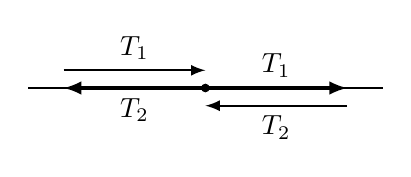
\begin{tikzpicture}[>=latex, scale=.9]
\draw[very thick, <->] (2,0)--node[above]{$T_1$}(0,0)--node[below]{$T_2$}(-2,0);
\draw[thick, ->](2,-.25)--node[below]{$T_2$}(0,-.25);
\draw[thick, ->](-2,.25)--node[above]{$T_1$}(0,.25);
\draw(0,0)[fill=black]circle (1.5pt);
\draw(-2.5,0)--(2.5,0);
    \end{tikzpicture}
    \caption{}
    \end{minipage}
    \end{figure}

如果我们用$\Vec{AB}$, $\Vec{CD}$表示平面上点的平移,我们就说向量$\Vec{AB},\Vec{CD},\ldots$.印刷时
经常用粗体字$\bf{a}$、$\bf{b}$、$\bf{c}$等表
示一个向量.向量$\bf{a}$、$\bf{b}$、$\bf{c}$在
手写时常写作$\vec{a}$、$\vec{b}$、$\vec{c}$.

如果向量$\vec{a}$, 把$A$点移
动到$B$点,$C$点移动到$D$点,$E$点移动到$F$点(图3.10),则
\[\vec{a}=\Vec{AB}=\Vec{CD}=\Vec{EF}=\cdots\]
这些同向且等长的有向线段都表示同一个向量,也就是说它
们中的任一个都可用来表示向量$\vec{a}$.
\begin{figure}[htp]
    \centering
    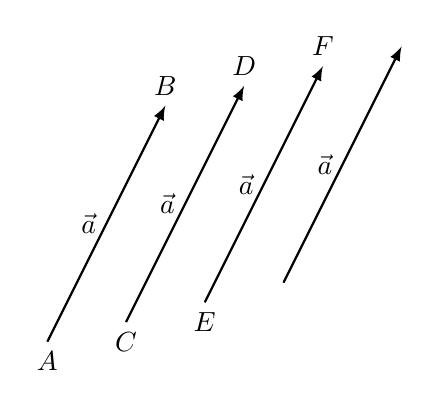
\begin{tikzpicture}[>=latex]
\draw[thick, ->](0,0)node[below]{$A$}--node[left]{$\vec{a}$}(1.5,3)node[above]{$B$};
\draw[thick, ->](1,0.25)node[below]{$C$}--node[left]{$\vec{a}$}(2.5,3.25)node[above]{$D$};
\draw[thick, ->](2,.5)node[below]{$E$}--node[left]{$\vec{a}$}(3.5,3+.5)node[above]{$F$};
\draw[thick, ->](3,.75)--node[left]{$\vec{a}$}(4.5,3+.75);        
    \end{tikzpicture}

    \caption{}
\end{figure}


若$\vec{a}=\Vec{AB}$, 则$\Vec{AB}$的长叫做$\vec{a}$的长度,记作$|\Vec{AB}|$或$|\vec{a}|$.
射线$\Vec{AB}$的方向叫做向量$\vec{a}$的方向.零平移又叫做\textbf{零向量},它
的方向不确定.

如果$\Vec{AB}$与$\Vec{CD}$的方向相同,那么$\Vec{AB}$, $\Vec{CD}$叫做\textbf{同向
向量},如果$\Vec{A_1B_1}$、$\Vec{C_1D_1}$的方向相反,那么$\Vec{A_1B_1}$、$\Vec{C_1D_1}$叫
做\textbf{反向向量}(图3.11).方向相同或相反的向量,叫做\textbf{平行
向量}.
\begin{figure}[htp]
    \centering
\begin{tikzpicture}[>=latex]
\begin{scope}
    \draw[thick, ->] (0,0)node[below]{$A$}--(0,3)node[above]{$B$};
    \draw[thick, ->] (1,.5)node[below]{$C$}--(1,2.5)node[above]{$D$};    
    \draw[thick, ->] (2,1)--node[left]{$\vec{a}$}(2,3);
\end{scope}
\begin{scope}[xshift=5cm]
    \draw[thick, ->] (0,0)node[below]{$A_1$}--(0,3)node[above]{$B_1$};
    \draw[thick, <-] (1,.5)node[below]{$D_1$}--(1,3)node[above]{$C_1$};    
    \draw[thick, <-] (2,1)--node[left]{$\vec{b}$}(2,2.5);
\end{scope}
\end{tikzpicture}
    \caption{}
\end{figure}

长度为1个单位的向量叫做\textbf{单位向量},通常我们用单位
向量表示平面上的一个方向.

以后我们用到记号$\Vec{AB}$或$\vec{a}$, 它们表示的是一个有向线段
还是一个向量,一般我们都不另加说明,读者可根据实际问
题加以区分.

\begin{ex}
\begin{enumerate}
    \item 用有向线段表示以下平移:
\begin{enumerate}
    \item $T_1$: 向东5cm;
    \item $T_2$: 向南偏西$30^{\circ}$, 3cm;
    \item $T_3$: 向北偏西$60^{\circ}$, 50km.
\end{enumerate}
\item  用有向线段表示以下两个平移的合成:
\begin{enumerate}
    \item $T_1$: 向西5里,$T_2$: 向南3里.
    \item $T_1$: 向北4里,$T_2$: 向西8里.
\end{enumerate}
\end{enumerate}
\end{ex}

\subsection{向量的加法与减法}
向量$\vec{a}$与$\vec{b}$的合成就叫做$\vec{a}$与
$\vec{b}$的和,记作$\vec{a}+\vec{b}$, 即
\[\vec{a}+\vec{b}=\vec{b}\circ \vec{a}\]

由上节定理可知,$\vec{a}$与$\vec{b}$的和$\vec{a}+\vec{b}$也是一个向量.由
于每个向量可由一点和它的象点所唯一确定,所以可按下面
方法作$\vec{a}+\vec{b}$.

在平面上,任取一点$A$ (图3.12), 作$\Vec{AB}=\vec{a}$, $\Vec{BC}=\vec{b}$, 即
$\vec{a}$与$\vec{b}$的合成把$A$点移动到$C$点,因而
\[\Vec{AC}=\vec{a}+\vec{b}\]
\begin{figure}[htp]
    \centering
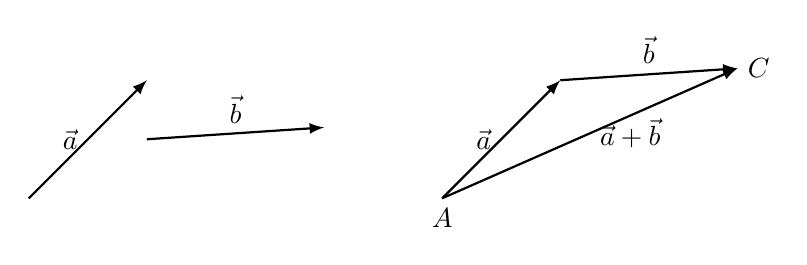
\begin{tikzpicture}[>=latex, scale=1.5]
\begin{scope}
    \draw[->,  thick](0,0)--node[left]{$\vec{a}$}(1,1);
    \draw[->,  thick] (1,.5)--node[above]{$\vec{b}$}(2.5,.6);
\end{scope}

\begin{scope}[xshift=3.5cm]
    \draw[->,  thick](0,0)node[below]{$A$}--node[left]{$\vec{a}$}(1,1);
    \draw[->,  thick](1,1)--node[above]{$\vec{b}$}(2.5,1.1)node[right]{$C$};
    \draw[->,  thick](0,0)--node[right]{$\vec{a}+\vec{b}$}(2.5,1.1);
\end{scope}
\end{tikzpicture}    
    \caption{}
\end{figure}

以上求和作图法叫做\textbf{三角形求和法则}.

由于平移的合成满足交换律,所以向量加法也满足交换
律,即
\[\vec{a}+\vec{b}=\vec{b}+\vec{a}\]

读者不难从图3.13
去验证,向量加法还满
足结合律,即
\[(\vec{a}+\vec{b})+\vec{c}=\vec{a}+(\vec{b}+\vec{c})\]
\begin{figure}[htp]\centering
    \begin{minipage}[t]{0.48\textwidth}
    \centering
\begin{tikzpicture}[>=latex,scale=1.5]
    \tkzDefPoints{0/0/A, 1/1.5/B, 3/1.7/C, 3.5/0/D}
\draw[->, thick](A)--node[left]{$\vec{a}$}(B);
\draw[->, thick](A)--node[above,rotate=30]{$\vec{a}+\vec{b}$}(C);
\draw[->, thick](A)--node[below]{$(\vec{a}+\vec{b})+\vec{c}=\vec{a}+(\vec{b}+\vec{c})$}(D);
\draw[->, thick](B)--node[above]{$\vec{b}$}(C);
\draw[->, thick](B)--node[above,rotate=-35]{$\vec{b}+\vec{c}$}(D);
\draw[->, thick](C)--node[right]{$\vec{c}$}(D);
    \end{tikzpicture}
    \caption{}
    \end{minipage}
    \begin{minipage}[t]{0.48\textwidth}
    \centering
    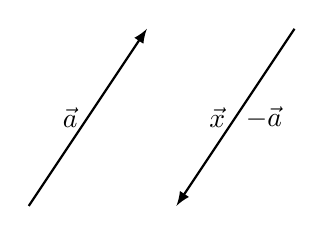
\begin{tikzpicture}[>=latex, scale=1.5]
      \draw[->, thick](0,0)--node[left]{$\vec{a}$}(1,1.5);
      \draw[<-, thick](1.25,0)--node[left]{$\vec{x}$}node[right]{$-\vec{a}$}(2.25,1.5);
    \end{tikzpicture}
    \caption{}
    \end{minipage}
    \end{figure}

容易看出,$\vec{a}+\vec{0}=\vec{0}+\vec{a}=\vec{a}$.

如果向量$\vec{a}$与$\vec{x}$反向且等长,那么由求和作图法可知
(图3.14)
\[\vec{a}+\vec{x}=\vec{0}\]

如果用$-\vec{a}$表示$\vec{x}$, 那么$-\vec{a}$叫
做$\vec{a}$的\textbf{逆向量}或\textbf{负向量},于是
\[\vec{a}+(-\vec{a})=\vec{0}\]
如图3.15所示.

\begin{figure}[htp]
    \centering
    \begin{minipage}[t]{0.48\textwidth}
    \centering
    \begin{tikzpicture}[>=latex, scale=1.4]
\tkzDefPoints{0/0/A, 3/0/B, 1.4/1.5/C, 0/1/A', 3.5/1/B'}
\tkzDefPointsBy[translation = from A to A'](C){C'}
\tkzDefPointsBy[translation = from B to B'](C){C''}
\draw[->, thick](A)--node[below]{$\vec{a}+(-\vec{b})$}(B);
\draw[->, thick](A)--node[left]{$\vec{a}$}(C);
\draw[->, thick](A')--node[left]{$\vec{a}$}(C');
\draw[<-, thick](B)--node[right]{$-\vec{b}$}(C);
\draw[->, thick](B')--node[right]{$\vec{b}$}(C'');

    \end{tikzpicture}
    \caption{}
    \end{minipage}
    \begin{minipage}[t]{0.48\textwidth}
    \centering
    \begin{tikzpicture}[>=latex, scale=1.4]
\tkzDefPoints{0/0/A, 3/0/B, 3.7/2/C}
\tkzDefPointsBy[translation = from B to C](A){D}
\tkzDrawSegments[->](D,C B,C D,B)
\tkzDrawSegments(A,C)
\tkzInterLL(A,C)(B,D)  \tkzGetPoint{O}
\draw(A)--node[above]{$\vec{a}+\vec{b}$}(O);
\draw(O)--node[above]{$\vec{a}-\vec{b}$}(B);

\draw[->](A)--node[below]{$\vec{a}$}(B);
\draw[->](A)--node[left]{$\vec{b}$}(D);
\tkzLabelPoints[below](A,B)
\tkzLabelPoints[above](C,D)

    \end{tikzpicture}
    \caption{}
    \end{minipage}
  \end{figure}

\begin{example}
已知:$\parallelogram ABCD$, $\Vec{AB}=\vec{a}$,$\Vec{AD}=\vec{b}$(图3.16).

求证:$\Vec{AC}=\vec{a}+\vec{b},\qquad \Vec{DB}=\vec{a}-\vec{b}$
\end{example}

\begin{proof}
因为$\Vec{AC}=\Vec{AB}+\Vec{BC},\; \Vec{BC}=\Vec{AD}$,所以
\[\Vec{AC}=\Vec{AB}+\Vec{AD}=\vec{a}+\vec{b}\]
又因为$\Vec{DB}=\Vec{DC}+\Vec{CB},\quad \Vec{DC}=\vec{a},\quad \Vec{CB}=-\vec{b}$

所以$\Vec{DB}=\vec{a}-\vec{b}$
\end{proof}    

由例3.4可知,位于一个平行四边形的一条“对角线向量”等于相邻两个“边向量”之和,而另一条“对角线向量”等于相邻两个“边向量”之差,由此,我们还可得到求两个向量和与差的方法如下:

\begin{blk}
   {求和的平行四边形法则} 已知$\vec{a}$、$\vec{b}$, 任取一点$A$, 作$\Vec{AB}=\vec{a}$, $\Vec{AD}=\vec{b}$, 再以$\Vec{AB}$、$\Vec{AD}$为边作$\parallelogram ABCD$, 则对角线上的向量$\Vec{AC}$就是$\vec{a}$与$\vec{b}$之和,即
   \[\vec{a}+\vec{b}=\Vec{AB}+\Vec{AD}=\Vec{AC}\] 
\end{blk}

\begin{blk}
    {求$\vec{a}-\vec{b}$的三角形法则} 已知$\vec{a}$、$\vec{b}$, 在平面上任取一点$A$, 作$\Vec{AB}=\vec{a}$, $\Vec{AD}=\vec{b}$, \textbf{以减量$\vec{b}$的终点($D$)为始点,被减量$\vec{a}$的终点($B$)为终点的向量$\Vec{DB}$就是$\vec{a}-\vec{b}$}, 即
    \[\vec{a}-\vec{b}=\Vec{AB}-\Vec{AD}=\Vec{DB}\] 
\end{blk}

对于多个向量$\vec{a}_1,\vec{a}_2,\ldots,\vec{a}_n$的求和法则,可由三角形求和法则推广如下:

已知$\vec{a}_1,\vec{a}_2,\ldots,\vec{a}_n$,在平面上任取一点$O$, 作$\Vec{OA_1}=\vec{a}_1$, 然后在$A_1$上引$\Vec{A_1A_2}=\vec{a}_2$, 再在$A_2$上引$\Vec{A_2A_3}=\vec{a}_3$, 如此下去,我们由这$n$条向量构成一条折线,由两个向量的求和
法则,我们可推知,以第一条有向线段的始点为始点,最后一条有向线段的终点为终点的有向线段所表示的向量就是这
$n$个向量之和,在图3.17中,
\[\vec{a}_1+\vec{a}_2+\vec{a}_3+\vec{a}_4=\Vec{OA_1}+\Vec{A_1A_2}+\Vec{A_2A_3}+\Vec{A_3A_4}=\Vec{OA_4}\]

\begin{figure}[htp]
    \centering
    \begin{minipage}[t]{0.48\textwidth}
    \centering
    \begin{tikzpicture}[>=latex, scale=1.5]
\tkzDefPoints{0/0/O, .5/1/A_1, 1.5/1.5/A_2, 2.5/1/A_3, 3/0/A_4}
\draw[->, thick](O)--node[left]{$\vec{a}_1$}(A_1);
\draw[->, thick](O)--node[below]{$\vec{a}_1+\vec{a}_2+\vec{a}_3+\vec{a}_4$}(A_4);
\draw[->, thick](A_1)--node[above]{$\vec{a}_2$}(A_2);
\draw[->, thick](A_2)--node[above]{$\vec{a}_3$}(A_3);
\draw[->, thick](A_3)--node[right]{$\vec{a}_4$}(A_4);
    \end{tikzpicture}
    \caption{}
    \end{minipage}
    \begin{minipage}[t]{0.48\textwidth}
    \centering
    \begin{tikzpicture}[>=latex, scale=.7]
\draw(-2,0)--(5,0);
\draw[->](0,-4.5)--(0,3)node[left]{北};
\draw[->, thick](0,0)--node[below]{$\vec{a}$}(2,0)node[below]{$A$};
\draw[->, thick](0,0)--node[above]{$\vec{b}$}(-1,0)node[below]{$B$};
\node at (0,0)[below left]{$O$};
\draw[->, thick](2,0)--node[below]{$\vec{a}$}(4,0)node[below]{$E$};
\draw[->, thick](0,0)--(0,2)node[left]{$C$};
\draw[->, thick](0,-2)--node[right]{$\vec{d}$}(0,-4)node[left]{$D$};
\draw[->, thick](0,0)--(0,-2)node[left]{$H$};
\draw[->, thick](0,0)--(1,0)node[above]{$F$};
\draw[->, thick](0,0)--(2,2)node[above]{$G$};
\draw[->, thick](2,0)--node[right]{$\vec{c}$}(2,2);


    \end{tikzpicture}
    \caption{}
    \end{minipage}
  \end{figure}

\begin{example}
已知:$\vec{a}=$“向东10km”,$\vec{b}=$“向西5km”,$\vec{c}=$“向北10km”,$\vec{d}=$“向南20km”,求:$\vec{a}+\vec{a}$, $\vec{a}+\vec{b}$, $\vec{a}+\vec{c}$, $\vec{c}+\vec{d}$.
\end{example}

\begin{solution}
如图3.18所示,作$\Vec{OA}=\vec{a}$, $\Vec{OB}=\vec{b}$, $\Vec{OC}=\vec{c}$, $\Vec{OD}=\vec{d}$,则:
\[\begin{split}
    \Vec{OE}&=\vec{a}+\vec{a}=\text{“向东20km”}\\
    \Vec{OF}&=\vec{a}+\vec{b}=\text{“向东5km”}\\
    \Vec{OG}&=\vec{a}+\vec{c}=\text{“向东北$10\sqrt{2}$km”}\\
    \Vec{OH}&=\vec{c}+\vec{d}=\text{“向南10km”}   
\end{split}\]
\end{solution}

由例3.5, 我们可以看出,两个方向相同的向量相加时,它们的和向量的方向与已知两个向量的方向相同,其长度等于它们的长度之和,两个方向相反的向量相加时,它们的和向量的方向与长度较长的那个向量方向相同,其长度等于两个向量长度差的绝对值.  

\subsubsection*{练习}

\begin{enumerate}
    \item 作出下列各组向量的和:
\begin{figure}[htp]
  \centering
  \begin{tikzpicture}[>=latex]
\begin{scope}[scale=.8]
\draw[<->, thick](3,2.2)--node[above]{$\vec{b}$}(0,0)--node[below]{$\vec{a}$}(-2,2);    
\end{scope}
\begin{scope}[xshift=5cm, scale=.8]
    \draw[->, thick](0,3)--node[left]{$\vec{a}$}(0,1);
\draw[->, thick](0,1)--node[below]{$\vec{b}$}(2.5,1);
\end{scope}
\begin{scope}[yshift=-3cm, xshift=-2cm]
      \draw[->, thick](0,1)--node[above]{$\vec{a}$}(2.5,1.5);
\draw[<-, thick](0,0)--node[above]{$\vec{b}$}(2,-.5);
\end{scope}
\begin{scope}[xshift=1.5cm, yshift=-3cm]
 \draw[->, thick](0,2)--node[right]{$\vec{b}$}(2.5,0);
\draw[<-, thick](-0.2,0)--node[left]{$\vec{a}$}(2,2);    
\end{scope}
\begin{scope}[xshift=5cm, yshift=-3cm]
    \draw[->, thick](0,.7)--node[above]{$\vec{a}$}(1.5,.7);
\draw[->, thick](0,0)--node[below]{$\vec{b}$}(2.5,0);      
\end{scope}
\begin{scope}[xshift=1cm, yshift=-6cm]
    \draw[<->, thick](-2.5,0)--node[above]{$\vec{b}$}(0,0)--node[above]{$\vec{a}$}(2,0);
  \tkzDrawPoint(0,0)
\end{scope}
\begin{scope}[xshift=4cm, yshift=-6cm]
    \draw[->, thick](0,0)--node[left]{$\vec{a}$}(2,1.8);
  \draw[->, thick](2,1)--node[above right]{$\vec{b}$}(4.5,1);
  \draw[->, thick](2.5,1.5)--node[below left]{$\vec{c}$}(4,-.5);
\end{scope}
  \end{tikzpicture}
\end{figure}

\item 求$\vec{a}-\vec{b}$
\begin{figure}[htp]
    \centering
    \begin{minipage}[t]{0.48\textwidth}
    \centering
    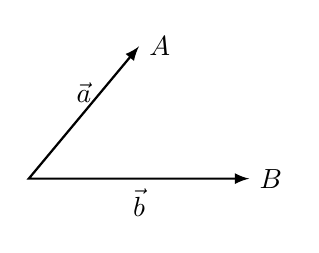
\begin{tikzpicture}[>=latex, scale=1.4]
\draw[<->, thick](1,1.2)node[right]{$A$}--node[above]{$\vec{a}$}(0,0)--node[below]{$\vec{b}$}(2,0)node[right]{$B$};
  \end{tikzpicture}
  \caption*{(1)}
    \end{minipage}
    \begin{minipage}[t]{0.48\textwidth}
    \centering
    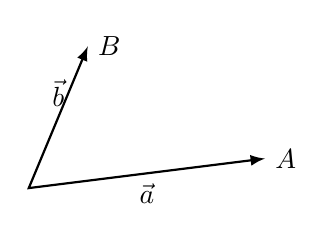
\begin{tikzpicture}[>=latex, scale=1.5]
\draw[<->, thick](.5,1.2)node[right]{$B$}--node[above]{$\vec{b}$}(0,0)--node[below]{$\vec{a}$}(2,0.25)node[right]{$A$};  
    \end{tikzpicture}
    \caption*{(2)}
    \end{minipage}
  \end{figure}

  \begin{figure}[htp]
    \centering
    \begin{minipage}[t]{0.48\textwidth}
    \centering
    \begin{tikzpicture}[>=latex, scale=1]
  \draw[->, thick](0,0)--node[above]{$\vec{b}$}(4,0);
  \draw[->, thick](0.5,-.5)--node[above]{$\vec{a}$}(1.5,2);
    \end{tikzpicture}
    \caption*{(3)}
    \end{minipage}
    \begin{minipage}[t]{0.48\textwidth}
    \centering
    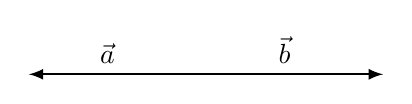
\begin{tikzpicture}[>=latex, scale=1]
        \draw[<->, thick](-2,0)--node[above]{$\vec{a}$}(0,0)--node[above]{$\vec{b}$}(2.5,0);
        \tkzDrawPoint(0,0)
    \end{tikzpicture}
    \caption*{(4)}
    \end{minipage}
  \end{figure}


    \item 任给两个向量$\vec{a}$、$\vec{b}$,用平行四边形法则求$\vec{a}+\vec{b}$.
    \item 已知$\triangle ABC$, 求证:$\Vec{AB}+\Vec{BC}+\Vec{CA}=0$.
    \item 如果三个向量$\vec{a}$、$\vec{b}$、$\vec{c}$, 满足$\vec{a}+\vec{b}+\vec{c}=0$, 问表示这三个向量的有向线段能否构成三角形.

\end{enumerate}

\subsection{$n$个$\vec{a}$连加之和}

\begin{blk}{定义}
如果$n$是正整数,定义
\[\underbrace{\vec{a}+\vec{a}+\vec{a}+\cdots+\vec{a}}_{\text{$n$个}}=n\vec{a}\] 
\end{blk}

例如,$\vec{a}+\vec{a}+\vec{a}+\vec{a}=4\vec{a}$.

\begin{example}
如$n,m$为正整数,试证:
\begin{enumerate}
    \item $n\left(m\vec{a}\right)=(mn)\vec{a}$
    \item $n\left(\vec{a}+\vec{b}\right)=n\vec{a}+n\vec{b}$(分配律)
\end{enumerate}
\end{example}   

\begin{proof}
\begin{enumerate}
    \item 
\[\begin{split}
     n\left(m\vec{a}\right)&=\overbrace{m\vec{a}+m\vec{a}+\cdots +m\vec{a}}^{n\text{个}}\\
&=\underbrace{\underbrace{\vec{a}+\vec{a}+\cdots+\vec{a}}_{m\text{个}}+\underbrace{\vec{a}+\vec{a}+\cdots+\vec{a}}_{m\text{个}}+\cdots +\underbrace{\vec{a}+\vec{a}+\cdots+\vec{a}}_{m\text{个}}}_{n\text{个}}\\
&=(nm)\vec{a} 
\end{split}\]
\item 
\[\begin{split}
     n\left(\vec{a}+\vec{b}\right)&=\overbrace{\left(\vec{a}+\vec{b}\right)+\left(\vec{a}+\vec{b}\right)+\cdots +\left(\vec{a}+\vec{b}\right)}^{n\text{个}}\\
   &=  \underbrace{\vec{a}+\vec{a}+\cdots+\vec{a}}_{n\text{个}}+\underbrace{\vec{b}+\vec{b}+\cdots+\vec{b}}_{n\text{个}}\\
     &=n\vec{a}+n\vec{b}
\end{split}\]
\end{enumerate}    
\end{proof}

下面让我们来分析一下$n\left(\vec{a}+\vec{b}\right)=n\vec{a}+n\vec{b}$的几何意义:取$\Vec{AB}=\vec{a}$, $\Vec{BC}=\vec{b}$ (图3.19), 则$\vec{a}+\vec{b}=\Vec{AC}$, 再取$\Vec{AB'}=n\vec{a}$, 过$B'$点作$BC$的平行线,取$B'C'$和$\Vec{DC}$同向且其长是$|\Vec{BC}|$的$n$倍,即$\Vec{B'C'}=n\vec{b}$, 由上述分配律有:
\[\Vec{AC'}=\Vec{AB'}+\Vec{B'C'}=n\vec{a}+n\vec{b}=n\left(\vec{a}+\vec{b}\right)=n\Vec{AC}\]
由此可知,$A$、$C$、$C'$三点共线并且$\Vec{AC'}$的长度是$\Vec{AC}$长度的$n$倍.这就证明了相似三角形基本定理(即\textbf{两个三角形中,如果有三个角对应相等,那么它们的三边就对应成比例}).

反之,如果$\triangle ABC\backsim \triangle AB'C'$且
$\frac{\overline{AB'}}{\overline{AB}}=n$,
则由相似三角形定理有
\[\Vec{AB'}=n\Vec{AB},\qquad \Vec{B'C'}=n\Vec{BC},\qquad \Vec{AC'}=n\Vec{AC}\]
\[\begin{split}
    \Vec{AC'}&=n\Vec{AC}=n\left(\Vec{AB}+\Vec{BC}\right)\\
    \Vec{AC'}&=\Vec{AB'}+\Vec{B'C'}=n\Vec{AB}+n\Vec{BC}
\end{split}\]
故得
\[n\left(\Vec{AB}+\Vec{BC}\right)=n\Vec{AB}+n\Vec{BC}\]
这就证明了上述分配律成立.

总结上面的分析,我们可以看到,运算律$n(\vec{a}+\vec{b})=
=n\vec{a}+n\vec{b}$和相似比为整数的相似三角形定理是同一几何事实的两种表达形式,它们在逻辑上具有等价关系.我们还可以把$n(\vec{a}+\vec{b})=
=n\vec{a}+n\vec{b}$的代数证明和边长之比为$n$的相似三角形定理的几何证明再加以分析比较.为清楚起见,我们取$n=3$ (图3.19).

\begin{figure}[htp]
    \centering
    \begin{minipage}[t]{0.58\textwidth}
    \centering
    \begin{tikzpicture}[>=latex, scale=1]
\tkzDefPoints{0/0/A, 5/0/B', 6/3/C'}
\tkzDefPointWith[linear, K=.333](A,C') \tkzGetPoint{C}
\tkzDefPointWith[linear, K=.333](A,B') \tkzGetPoint{B}
\tkzDefPointWith[linear, K=.333](B',C') \tkzGetPoint{D''}
\tkzDefPointWith[linear, K=.667](A,C') \tkzGetPoint{C''}
\tkzDefPointWith[linear, K=.667](A,B') \tkzGetPoint{B''}
\tkzDefPointWith[linear, K=.667](B',C') \tkzGetPoint{D'}
\tkzDrawSegments[thick, ->](A,C A,B A,B' B',C')
\tkzDrawSegments(A,C' C,D'' C'',D' C,B C'',B'')
\tkzDrawSegments[dashed](B,D')
\tkzLabelPoints[below](A,B,B')
\tkzLabelPoints[above](C,C')

\tkzInterLL(B'',C'')(C,D'')  \tkzGetPoint{O}

\draw(A)--node[below]{$\vec{a}$}(B);
\draw(A)--node[above left]{$\vec{a}+\vec{b}$}(C);
\draw(C)--node[above]{$\vec{a}$}(O);
\draw(C'')--node[above]{$\vec{a}$}(D');
\draw(C)--node[right]{$\vec{b}$}(B);
\draw(C'')--node[right]{$\vec{b}$}(O); 
    \end{tikzpicture}
    \caption{}
    \end{minipage}
    \begin{minipage}[t]{0.38\textwidth}
    \centering
    \begin{tikzpicture}[>=latex, scale=1]
\tkzDefPoints{0/0/A, 0/.6/A_1, 0/1.2/A_2, 0/2.4/A_{n-1}, 0/3.3/B}
\tkzDrawSegments[->](A,B)
\tkzLabelPoints[left](A_1,A_2,A_{n-1})
\tkzDrawPoints(A_1,A_2,A_{n-1})
\tkzLabelPoints[below](A)
\tkzLabelPoints[above](B)
    \end{tikzpicture}
    \caption{}
    \end{minipage}
  \end{figure}


\begin{proof}
\textbf{代数证明}
\begin{align*}
3 \left(\vec{a}+\vec{b}\right) &= \left(\vec{a}+\vec{b}\right)+\left(\vec{a}+\vec{b}\right)+\left(\vec{a}+\vec{b}\right)  \tag{用一次交换律}\\
&=\vec{a}+\vec{a}+\vec{b}+\vec{b}+\vec{a}+\vec{b} \tag{用两次交换律}\\
&= \vec{a}+\vec{a}+\vec{a}+\vec{b}+\vec{b}+\vec{b} =3\vec{a}+3\vec{b}
\end{align*}

\textbf{几何证明:}
主要是用平行分割把$\triangle AB'C'$分割成$3^2=9$个和$\triangle ABC$全等的小三角形来证明相似三角形定理(参看第二册第三章).
\end{proof}

比较上述代数证明和几何证明,可以看出,代数证明不需要作辅助线,比较简单明了.有意思的是几何证明中出现了三个平行四边形,应用了三次平行四边形定理,这正好与代数证明中应用了三次交换律相对应.

设$\Vec{AB}=\vec{a}$(图3.20),将$\overline{AB}$等分为$n$段:$\overline{AA_1},\overline{A_1A_2},\overline{A_2A_3},\ldots,\overline{A_{n-1}B}$,则有
\[\Vec{AA_1}=\Vec{A_1A_2}=\Vec{A_2A_3}=\cdots=\Vec{A_{n-1}B}\]
所以
\[n\Vec{AA_1}=\Vec{AA_1}+\Vec{A_1A_2}+\Vec{A_2A_3}+\cdots+\Vec{A_{n-1}B}=\Vec{AB}=\vec{a}\]
我们把上述$\Vec{AA_1}$定义为$\frac{1}{n}\vec{a}$,再者,我们把$\frac{m}{n}\vec{a}$定义为$\frac{1}{n}\left(m\vec{a}\right)$,其性质为
\[n\left(\frac{m}{n}\vec{a}\right)=m\vec{a}\]


\begin{example}
    试证
\begin{enumerate}
    \item $\frac{m}{n}\left(\frac{p}{q}\vec{a}\right)=\left(\frac{m}{n}\frac{p}{q}\right)\vec{a}$
    \item $\frac{n}{m}\left(\vec{a}+\vec{b}\right)=\frac{n}{m}\vec{a}+\frac{n}{m}\vec{b}$
\end{enumerate}
\end{example}

\begin{proof}
\begin{enumerate}
    \item 等式左边乘以$qn$,由例3.7得
\[\begin{split}
qn\left[\frac{m}{n}\left(\frac{p}{q}\vec{a}\right)\right]=q\left[n\frac{m}{n}\left(\frac{p}{q}\vec{a}\right)\right]&=(qm)\left(\frac{p}{q}\vec{a}\right)\\
&=m\left[q\left(\frac{p}{q}\vec{a}\right)\right]\\
&=\left(mp\vec{a}\right)=(mp)\vec{a}
\end{split}\]
再由上述有理数乘向量的定义即可得
\[\frac{m}{n}\left(\frac{p}{q}\vec{a}\right)=\frac{mp}{nq}\vec{a}=\left(\frac{m}{n}\cdot \frac{p}{q}\right)\vec{a}\]

\item 令$\vec{a}'=\frac{1}{m}\vec{a}$, $\vec{b}'=\frac{1}{m}\vec{b}$,则由例3.7可得
\[\begin{split}
    \frac{n}{m}\left(\vec{a}+\vec{b}\right)=\frac{n}{m}\left(m\vec{a}'+m\vec{b}'\right)&=\frac{n}{m}m\left(\vec{a}'+\vec{b}'\right)\\
&=n\left(\vec{a}'+\vec{b}'\right)\\
&=n\left(\frac{1}{m}\vec{a}+\frac{1}{m}\vec{b}\right)
=\frac{n}{m}\vec{a}+\frac{n}{m}\vec{b}
\end{split}\]
\end{enumerate}
\end{proof}

\begin{ex}
\begin{enumerate}
    \item 如何定义$(-1)\vec{a}$, $(-2)\vec{a}$和$(-n)\vec{a}$,才能使得例3.7中的两式对任何正负整数都能成立.
    \item 如何定义$\left(-\frac{1}{2}\right)\vec{a}$, $\left(-\frac{2}{3}\right)\vec{a}$和$\left(-\frac{m}{n}\right)\vec{a}$才能使例3.8中的两式对任何正负分数都成立.
    \item 比较本节例3.7、例3.8, 及上面练习1、2和初中第一册对于指数法则的逐步推广.
\end{enumerate}   
\end{ex}

\section*{习题3.1}
\addcontentsline{toc}{subsection}{习题3.1}

\begin{enumerate}
    \item 已知$\parallelogram{ABCD}$. $\Vec{AB}=\vec{a}$, $\Vec{AD}=\vec{b}$, $|\vec{a}|=3$,
$|\vec{b}|=5$, $\angle BAD=120^{\circ}$,求$\vec{a}+\vec{b}$与$\vec{a}-\vec{b}$之长.
\item 已知$\Vec{OA}$, $\Vec{OB}$且$|\Vec{OA}|=4$cm, $|\Vec{OB}|=5$cm, $\angle AOB=60^{\circ}$, 求$\Vec{OA}+\Vec{OB}$.
\item 在第2题中,让$\Vec{OA}$, $\Vec{OB}$的长不变,只有$\angle AOB$在变化,求$\Vec{OA}+\Vec{OB}$之长的最大值与最小值.

\item 如果不附加条件,任给一个向量$\vec{a}$, 你能把它分解为多少对向量之和?如果分解$\vec{a}$为两个向量之和且使这两个向量分别与已知两个向量$\vec{b}$、$\vec{c}$平行,这种分解是唯一的吗?
\end{enumerate}

\section{相似与向量的倍积}
\subsection{向量的倍积与运算律}

在初中,我们学习了相似这个基本概念,直观地说,相似就是放大或缩小,把相似和位移向量相结合,就可引出下述向量倍积的定义.

\begin{blk}
    {定义} 已知$\vec{a}$和实数$\lambda$, $\vec{a}$与实数$\lambda$ 的乘积$\lambda \vec{a}$ (或$\vec{a}\lambda $) 是一个向量,它的长是$|\lambda| \left|\vec{a}\right|$, 它的方向,当$\lambda >0$时与$\vec{a}$同向,当$\lambda <0$时与$\vec{a}$反向(图3.21); 对于0乘$\vec{a}$, 规定$0\vec{a}=0$, $\lambda \vec{a}$中的数量$\lambda$叫做$\vec{a}$的系数,$\lambda\vec{a}$叫做$\vec{a}$的倍积.
\end{blk}

\begin{figure}[htp]
    \centering
\begin{tikzpicture}[>=latex]
\draw[->, thick](0,0)--node[left]{$\tfrac{1}{2}\vec{a}$}(70:.5);
\draw[->, thick](1,0)--node[left]{${2}\vec{a}$}+(70:2);
\draw[->, thick](2,0)--node[left]{$\vec{a}$}+(70:1);
\draw[->, thick](3,0)--node[left]{$3\vec{a}$}+(70:3);
\draw[<-, thick](4,0)--node[left]{$-\vec{a}$}+(70:1);
\draw[<-, thick](5,0)--node[left]{$-3\vec{a}$}+(70:3);
\draw[<-, thick](6,0)--node[right]{$-\tfrac{1}{2}\vec{a}$}+(70:.5);
\end{tikzpicture}
    \caption{}
\end{figure}

\begin{blk}
    {定理} 向量的倍积满足如下的运算律,对$\lambda,\mu\in\mathbb{R}$,
\begin{enumerate}
    \item (分配律)$(\lambda+\mu)\vec{a}=\lambda\vec{a}+\mu\vec{a}$
    \item (结合律)$\lambda\left(\mu\vec{a}\right)=(\lambda\mu)\vec{a}$
    \item (分配律)$\lambda\left(\vec{a}+\vec{b}\right)=\lambda\vec{a}+\lambda\vec{b}$
\end{enumerate}    
\end{blk}

\begin{figure}[htp]
    \centering
\begin{tikzpicture}[>=latex]
\begin{scope}[scale=1]
\tkzDefPoints{0/-2/A, 2/-2/B, 4.5/-2/B', 2/-1/C, 4.5/.25/C'}
\tkzLabelPoints[below](A,B,B')
\tkzLabelPoints[above](C,C')
\draw[->, thick](A)--node[below]{$\vec{a}$}(B);
\draw[->, thick](B)--node[below]{$\lambda\vec{a}$}(B');
\draw[->, thick](B)--node[right]{$\vec{b}$}(C);
\draw[->, thick](B')--node[right]{$\lambda\vec{b}$}(C');
\draw[->, thick](A)--node[above]{$\vec{a}+\vec{b}$}(C);
\draw[->, thick](C)--node[above]{$\lambda\left(\vec{a}+\vec{b}\right)$}(C');
\node at (2.3, -3){$\lambda>0$};
\end{scope}
\begin{scope}[xshift=8cm, scale=.7]
\tkzDefPoints{0/0/A, -2/-1.5/B', 0/-3/C'}
\tkzDefPointWith[linear, K=2.1](B',A) \tkzGetPoint{B}
\tkzDefPointWith[linear, K=2.1](C',A) \tkzGetPoint{C}
\tkzLabelPoints[above](B,C)
\tkzLabelPoints[below](B',C')
\tkzLabelPoints[right](A)
\draw[->, thick](A)--node[below]{$\vec{a}$}(B);
\draw[->, thick](A)--node[above]{$\lambda\vec{a}$}(B');
\draw[->, thick](B)--node[above]{$\vec{b}$}(C);
\draw[->, thick](B')--node[below]{$\lambda\vec{b}$}(C');
\draw[->, thick](A)--node[left]{$\vec{a}+\vec{b}$}(C);
\draw[->, thick](A)--node[right]{$\lambda\left(\vec{a}+\vec{b}\right)$}(C');
\node at (0, -4){$\lambda<0$};
\end{scope}
\end{tikzpicture}
    \caption{}
\end{figure}



\begin{proof}
1、2两式读者可依倍积定义自己证明,证明现让我们应用相似形定理来证明3.

设$\Vec{AB}=\vec{a}$, $\Vec{BC}=\vec{b}$, 则$\Vec{AC}=\vec{a}+\vec{b}$, 在直线$AB$上取$B'$使$\Vec{AB'}=\lambda\Vec{AB}$, 过$B'$点作$BC$的平行线交直线$AC$于$C'$点($\lambda>0$, $\lambda<0$这两种情形如图3.22所示),不难由相似三角形定理得知:
\[\frac{\overline{AC'}}{\overline{AC}}=\frac{\overline{B'C'}}{\overline{BC}}=\frac{\overline{AB'}}{\overline{AB}}=\lambda\]
容易看出,当
\begin{enumerate}
    \item $\lambda>0$时,$\Vec{AC'}$与$\Vec{AC}$同向,$\Vec{B'C'}$与$\Vec{BC}$同向;
    \item $\lambda<0$时,$\Vec{AC'}$与$\Vec{AC}$反向,$\Vec{B'C'}$与$\Vec{BC}$反向. 
\end{enumerate}
所以
\[\Vec{B'C'}=\lambda\vec{b},\qquad \Vec{AC'}=\lambda\Vec{AC}=\lambda\left(\vec{a}+\vec{b}\right)\]
又:$\Vec{AC'}=\Vec{AB'}+\Vec{B'C'}=\lambda \vec{a}+\lambda\vec{b}$,故得:
\[\lambda\left(\vec{a}+\vec{b}\right)=\lambda \vec{a}+\lambda\vec{b}\]
\end{proof}

\begin{example}
计算下列各式
\begin{enumerate}
    \item $(-2)\x\frac{1}{2}\vec{a}$
    \item $2\left(\vec{a}+\vec{b}\right)-3\left(\vec{a}-\vec{b}\right)$
    \item $(\lambda+\mu)\left(\vec{a}+\vec{b}\right)-(\lambda-\mu)\left(\vec{a}-\vec{b}\right)$
\end{enumerate}
\end{example}

\begin{solution}
\begin{enumerate}
    \item $(-2)\x\frac{1}{2}\vec{a}=\left[(-2)\x\frac{1}{2}\right]\vec{a}=-\vec{a}$
    \item \[\begin{split}
        2\left(\vec{a}+\vec{b}\right)-3\left(\vec{a}-\vec{b}\right)=2\vec{a}+2\vec{b}-3\vec{a}+3\vec{b}&=\left(2\vec{a}-3\vec{a}\right)+\left(2\vec{b}+3\vec{b}\right)\\
        &=-\vec{a}+5\vec{b}
    \end{split}  \]
    \item \[\begin{split}
 &\qquad        (\lambda+\mu)\left(\vec{a}+\vec{b}\right)-(\lambda-\mu)\left(\vec{a}-\vec{b}\right)\\
&=\lambda \left(\vec{a}+\vec{b}\right)+\mu \left(\vec{a}+\vec{b}\right)-(\lambda-\mu)\vec{a}+(\lambda-\mu)\vec{b}\\
&=\lambda\vec{a}+\lambda \vec{b}+\mu \vec{a}+\mu \vec{b}-\lambda\vec{a}+\mu\vec{a}+\lambda\vec{b}-\mu \vec{b}\\
&=2\mu \vec{a}+2\lambda \vec{b}
\end{split}
\]
\end{enumerate}    
\end{solution}


\begin{example}
$\vec{a}$、$\vec{b}$为已知向量,且
$\frac{2}{3}\left(4\vec{a}-3\vec{c}\right)+3\left(5\vec{c}-4\vec{b}\right)=\vec{0}$,求$\vec{c}$.
\end{example}

\begin{solution}
原式可变形为:
\[\begin{split}
    \frac{8}{3}\vec{a}-2\vec{c}+15\vec{c}-12\vec{b}&=\vec{0}\\
    13\vec{c}&=12\vec{b}-\frac{8}{3}\vec{a}\\
    \vec{c}&=\frac{12}{13}\vec{b}-\frac{8}{39}\vec{a}
\end{split}\]
\end{solution}

\begin{example}
已知$\overline{AM}$是$\triangle ABC$的$\overline{BC}$边上的中线,若$\Vec{AB}=\vec{a}$, $\Vec{AC}=\vec{b}$,试用$\vec{a}$, $\vec{b}$表示$\Vec{AM}$. (图3.23)
\end{example}

\begin{figure}[htp]
    \centering
\begin{tikzpicture}[>=latex]
\tkzDefPoints{0/0/B, 1.5/0/M, 3/0/C, 2/2/A}
\tkzLabelPoints[below](B,M,C)
\tkzLabelPoints[above](A)
\tkzDrawSegments[->, thick](A,B A,M A,C B,M M,C)
\end{tikzpicture}
    \caption{}
\end{figure}

\begin{solution}
\[\begin{split}
    \Vec{AM}=\Vec{AB}+\Vec{BM}&=\Vec{AB}+\frac{1}{2}\Vec{BC}\\
&=\Vec{AB}+\frac{1}{2}\left(\Vec{AC}-\Vec{AB}\right)\\
&=\vec{a}+\frac{1}{2}\left(\vec{b}-\vec{a}\right)=\frac{1}{2}\left(\vec{a}+\vec{b}\right)
\end{split}\]
\end{solution}

\begin{ex}
\begin{enumerate}
    \item 化简下列各式:
\begin{enumerate}
    \item $4\left(2\vec{a}-3\vec{b}\right)+5\left(3\vec{a}-2\vec{b}\right)$
    \item $\frac{1}{4}\left(\vec{a}+2\vec{b}\right)-\frac{1}{6}\left(5\vec{a}-2\vec{b}\right)+\frac{1}{4}\vec{a}$
    \item $3\left(3\vec{a}-4\vec{b}+\vec{c}\right)-3\left(2\vec{a}+\vec{b}-3\vec{c}\right)$
\end{enumerate}
\item 用几何作图方法证明
$\frac{\vec{a}+\vec{b}}{2}+\frac{\vec{a}-\vec{b}}{2}=\vec{a}$.
\item 求未知向量$\vec{x}$
\begin{enumerate}
    \item $\vec{x}+2\left(\vec{a}+\vec{x}\right)=\vec{0}$
    \item $3\vec{a}+4\left(\vec{b}-\vec{x}\right)=\vec{0}$
    \item $2\left(\vec{x}-\frac{1}{3}\vec{a}\right)-\frac{1}{2}\left(\vec{b}-3\vec{x}+\vec{c}\right)+\vec{b}=\vec{0}$
\end{enumerate}
\item 如图,已知梯形$ABCD$, $AB\parallel CD$且$\overline{AB}=2\overline{DC}$, $M$、$N$分别是$\overline{DC}$、$\overline{AB}$的中点,设$\Vec{AB}=\vec{a}$, $\Vec{AD}=\vec{b}$, 试用$\vec{a}$, $\vec{b}$表示$\Vec{DC}$, $\Vec{BC}$, $\Vec{MN}$.
\item 如图,已知$\parallelogram OADB$是以向量$\Vec{OA}=\vec{a}$, $\Vec{OB}=\vec{b}$为邻边的平行四边形,又知$\Vec{BM}=\frac{1}{3}\Vec{BC}$, $\Vec{CN}=\frac{1}{3}\Vec{CD}$, 试用$\vec{a}$, $\vec{b}$表示$\Vec{OM}$, $\Vec{ON}$, $\Vec{MN}$.
\item 已知$\triangle ABC$的$\Vec{BC}=\vec{a}$, $\Vec{CA}=\vec{b}$, $\Vec{AB}=\vec{c}$, 三边$\overline{BC}$、$\overline{CA}$、$\overline{AB}$的中点依次为$D$、$E$、$F$, 试用$\vec{a},\vec{b},\vec{c}$表示$\Vec{AD}+\Vec{BE}+\Vec{CF}$.
\end{enumerate}
\end{ex}

\begin{figure}[htp]
    \centering
    \begin{minipage}[t]{0.48\textwidth}
    \centering
    \begin{tikzpicture}[>=latex, scale=1]
\tkzDefPoints{0/0/A, 4/0/B, 3.5/2.5/C, 1.5/2.5/D}
\tkzDefMidPoint(A,B)\tkzGetPoint{N}
\tkzDefMidPoint(C,D)\tkzGetPoint{M}
\tkzDrawSegments[->, thick](D,C M,N N,B B,C)
\tkzLabelPoints[above](C,D,M)
\tkzLabelPoints[below](A,B,N)
\draw[->, thick](A)--node[left]{$\vec{b}$}(D);
\draw[thick](A)--node[below]{$\vec{a}$}(N);
    \end{tikzpicture}
    \caption*{第4题}
    \end{minipage}
    \begin{minipage}[t]{0.48\textwidth}
    \centering
    \begin{tikzpicture}[>=latex, scale=1.3]
  \tkzDefPoints{0/0/O, 3/0/A, 4/2/D}
\tkzDefPointsBy[translation = from A to D](O){B}
\tkzInterLL(A,B)(O,D)  \tkzGetPoint{C}
\tkzDefPointWith[linear, K=.333](C,D) \tkzGetPoint{N}
\tkzDefPointWith[linear, K=.333](B,C) \tkzGetPoint{M}
\tkzDrawSegments(B,D A,D A,B O,D)
\tkzDrawSegments[->, thick](M,N O,M C,N B,M)
\draw[->, thick](O)--node[below]{$\vec{a}$}(A);
\draw[->, thick](O)--node[left]{$\vec{b}$}(B);


\tkzLabelPoints[below](A,O,C)
\tkzLabelPoints[above](B,D,M,N)
    \end{tikzpicture}
    \caption*{第5题}
    \end{minipage}
  \end{figure}

\subsection{平行向量与两个向量的线性关系}

\begin{blk}
    {平行向量基本定理} 如果向量$\vec{a}\ne \vec{0}$, 则$\vec{b}\parallel \vec{a}$的一个充要条件是存在一个唯一的实数$x$, 使$\vec{b}=x\vec{a}$.
\end{blk}

\begin{proof}
\begin{enumerate}
    \item 必要性:如果$\vec{a}\parallel \vec{b}$,$\vec{a}\ne \vec{0}$,可设$\frac{|\vec{b}|}{|\vec{a}|}=\mu$,
\begin{itemize}
    \item 若$\vec{b}$与$\vec{a}$同向,则令$x=\mu$,可得:
\[\vec{b}=\frac{|\vec{b}|}{|\vec{a}|}\vec{a}=x\vec{a}\]
    \item  若$\vec{b}$与$\vec{a}$反向,则令$x=-\mu$,可得:
\[\vec{b}=-\frac{|\vec{b}|}{|\vec{a}|}\vec{a}=x\vec{a}\]
\end{itemize}

唯一性,如果存在两个实数$x,x'$使$\vec{b}=x\vec{a}=x'\vec{a}$,则
\[(x-x')\vec{a}=\vec{0}\]
但$\vec{a}\ne \vec{0}$,所以$x-x'=0\quad \Rightarrow\quad x=x'$

\item 充分性,如果存在一实数$x$,使$\vec{b}=x\vec{a}$,根据向量倍积定义,则$\vec{a}$与$\vec{b}$方向相同或方向相反,因此:
\[\vec{b}\parallel \vec{a}\]
\end{enumerate}
\end{proof}

\begin{blk}
{推论} 两个向量$\vec{a}$, $\vec{b}$平行的充要条件是存在着两个不全为零的实数$x_1,x_2$使
\[x_1\vec{a}_1+x_2\vec{a}_2=\vec{0}\]
\end{blk}

\begin{proof}
\begin{enumerate}
    \item 必要性:如果$\vec{b}\parallel \vec{a}$, 对于$\vec{a}=\vec{b}=0$, 结论当然成立,假定$\vec{a}, \vec{b}$中有一个不是零向量,不妨设$\vec{a}\ne 0$, 由平行向量基本定理可知存在唯一的实数$x_1$, 使$\vec{b}=x_1\vec{a}$, 取$x_2=-1$, 则可写成
    \[x_1\vec{a}+x_2\vec{b}=\vec{0}\]
其中至少$x_2\ne 0$
\item 充分性:如果$x_1\vec{a}+x_2\vec{b}=\vec{0}$且$x_1,x_2$不全为零,不妨设$x_2\ne 0$, 于是可解出
\[\vec{b}=-\frac{x_1}{x_2}\vec{a}\]
所以:$\vec{a}\parallel \vec{b}$.
\end{enumerate}
\end{proof}

\begin{blk}
    {定义} 已知两个向量$\vec{a}_1$, $\vec{a}_2$, 如果存在着不全为零的两个实数$x_1,x_2$, 使
    \[x_1\vec{a}_1+x_2\vec{a}_2=\vec{0}\]
那么我们称$\vec{a}_1,\vec{a}_2$线性相关.
\end{blk}

由上面的推论可推知:\textbf{两个向量线性相关的充要条件是它们互相平行}.

\begin{blk}
    {定义} 如果$\vec{a}_1,\vec{a}_2$都是非零向量,且方程
    \[x_1\vec{a}_1+x_2\vec{a}_2=\vec{0}\]
仅当$x_1=x_2=0$时才成立,我们称向量$\vec{a}_1$与$\vec{a}_2$线性无关.
\end{blk}

由上面的推论可推知:\textbf{两个向量$\vec{a}_1,\vec{a}_2$线性无关的充要条件是它们不平行}.

\begin{ex}
\begin{enumerate}
    \item 用单位向量$\vec{e}$(即$|\vec{e}|=1$个单位)表示如下向量
\begin{enumerate}
    \item $\vec{a}$与$\vec{e}$的方向相同且它的长度是7个单位;
    \item $\vec{b}$与$\vec{e}$的方向相反且它的长度是5个单位;
    \item $\vec{c}$与$\vec{e}$的方向相反且它的长度是1/2个单位.
\end{enumerate} 
\item 问下列向量$\vec{a}$与$\vec{b}$的长度间和方向间有什么关系.
\begin{multicols}{2}
\begin{enumerate}
    \item $\vec{a}=-3\vec{b}$
    \item $\vec{a}=\frac{1}{2}\vec{b}$
    \item $2\vec{a}+3\vec{b}=\vec{0}$
    \item $3\vec{a}-5\vec{b}=\vec{0}$
    \item $\vec{a}=2\vec{e},\quad \vec{b}=4\vec{e}$
    \item $\vec{a}=\frac{1}{2}\vec{e},\quad \vec{b}=-4\vec{e}$
\end{enumerate}
\end{multicols}
\item 已知$\vec{a}+\vec{b}=3\vec{e}$, $\vec{a}-\vec{b}=5\vec{e}$, 问$\vec{a}$与$\vec{b}$是否平行?
\item 已知$\vec{a}_1=3\vec{e}$, $\vec{a}_2=-2\vec{e}$, 把$\vec{a}_1$、$\vec{a}_2$写成$x_1\vec{a}_1+x_2\vec{a}_2=\vec{0}$的形式.问$\vec{a}$与$\vec{b}$是否线性相关?
\item 在什么条件下$\vec{a}+\vec{b}$与$\vec{a}-\vec{b}$线性相关?
\item 若$\vec{a}\ne \vec{0}$, 试证明$x\vec{a}=\vec{0}\quad \Leftrightarrow\quad x=0$
\end{enumerate}  
\end{ex}

\section*{习题3.2}
\addcontentsline{toc}{subsection}{习题3.2}

\begin{enumerate}
    \item 把下列两个线性相关的向量写成$x\vec{a}+y\vec{b}=\vec{0}$的形式.
\begin{multicols}{3}
\begin{enumerate}
    \item $\vec{a}=\frac{1}{4}\vec{b}$
    \item $\vec{a}=2\vec{e},\quad \vec{b}=-3\vec{e}$
    \item $\vec{a}=-5\vec{e},\quad \vec{b}=3\vec{e}$
\end{enumerate}
\end{multicols}
\item 如果$\vec{a}=-2\vec{b}$, $\vec{c}=\frac{3}{5}\vec{a}-\vec{b}$, 问$\vec{a}$、$\vec{b}$、$\vec{c}$是否平行.
\item 解方程组中的$\vec{x}$, $\vec{y}$
\[\begin{cases}
    5\vec{x}+2\vec{y}=\vec{a}\\
    3\vec{x}-\vec{y}=\vec{b}
\end{cases}\]
\item 若 $x\vec{a}+y\vec{b}=\vec{0}$且$x+y=0$, 问$\vec{a}$及$\vec{b}$是否线性相关?
\item 已知$|\vec{a}|=3$, $\vec{b}$与$\vec{a}$反向且$|\vec{b}|=5$, 求$\vec{a}$与$\vec{b}$满足的向量关系式.
\item 设$A$、$B$、$C$、$D$是平面上任意四点,$M$、$N$分别为$\overline{AD}$与$\overline{BC}$的中点,求证:$2\Vec{MN}=\Vec{AB}+\Vec{DC}$.
\end{enumerate}

\section{长度、角度与内积运算}
\subsection{向量的内积}

已知两个非零向量$\vec{a}$、$\vec{b}$ (图3.24), 作$\Vec{OA}=\vec{a}$, $\Vec{OB}=\vec{b}$, $\angle AOB$就叫做$\vec{a}$与$\vec{b}$之间的夹角,记作$\expval{\vec{a},\vec{b}}$, $\expval{\vec{a},\vec{b}}$也就是向量$\vec{a}$与$\vec{b}$之间的方向差.

我们规定$0\le \expval{\vec{a},\vec{b}}\le \pi$, 在这个规定下,两个向量的夹角就被唯一确定了,并且$\expval{\vec{a},\vec{b}}=\expval{\vec{b},\vec{a}}$.

\begin{figure}[htp]
    \centering
    \begin{minipage}[t]{0.48\textwidth}
    \centering
    \begin{tikzpicture}[>=latex, scale=1]
        \tkzDefPoints{0/0/O, 2/0/A, 3/0/A'}
        \tkzDefPoint(50:2){B}
        \tkzDefPoint(50:3){B'}
        \tkzDrawSegments[dashed](B,B' A,A')
        \draw[thick,->](O)--node[below]{$\vec{a}$}(A);
        \draw[thick,->](O)--node[above]{$\vec{b}$}(B);
        \tkzLabelPoints[below](O,A)
        \tkzLabelPoints[above](B)
        \tkzMarkAngle[mark=none, size=.3](A,O,B)
    \end{tikzpicture}
    \caption{}
    \end{minipage}
    \begin{minipage}[t]{0.48\textwidth}
    \centering
    \begin{tikzpicture}[>=latex, scale=1.3]
\tkzDefPoints{0/0/B, 2/0/C, 3/1.5/A, 3.5/0/D}
\tkzLabelPoints[below](B,C)
\tkzLabelPoints[above](A)
\tkzMarkAngle[mark=none, size=.3](D,C,A)
\draw[thick,->](B)--node[below]{$\vec{a}$}(C);
\draw[thick,->](B)--node[left]{$\vec{a}+\vec{b}$}(A);
\draw[thick,->](C)--node[right]{$\vec{b}$}(A);
\tkzDrawSegments[dashed](C,D)
    \end{tikzpicture}
    \caption{}
    \end{minipage}
  \end{figure}

如果$\expval{\vec{b},\vec{a}}=\frac{\pi}{2}$, 那么称$\vec{a}$与$\vec{b}$互相\textbf{垂直},并记作$\vec{a}\bot \vec{b}$.由于零向量的方向是不确定的,所以零向量与任一向量的夹角也是不确定的,为了以后讨论问题方便,我们规定零向量与任一向量平行或垂直.

在平面几何中,一个重要的课题就是讨论三角形中的边角关系,其中最要紧的是余弦定理,如在$\triangle ABC$中,$\angle A$、$\angle B$、$\angle C$的对边长分别用$a$、$b$、$c$表示,则
\[c^2=a^2+b^2-2ab\cos\angle C\]

若设$\Vec{BC}=\vec{a}$,$\Vec{CA}=\vec{b}$,则
\[\Vec{BA}=\vec{a}+\vec{b},\quad |\vec{a}|=a,\quad |\vec{b}|=b,\quad |\vec{a}+\vec{b}|=c,\quad \expval{\vec{a},\vec{b}}=\pi-\angle C\]

上式换用向量的写法即可写为
\[|\vec{a}+\vec{b}|^2=|\vec{a}|^2+|\vec{b}|^2+2|\vec{a}|\cdot |\vec{b}|\cos\expval{\vec{a},\vec{b}}\]
或
\[|\vec{a}|\cdot |\vec{b}|\cos\expval{\vec{a},\vec{b}}=\frac{1}{2}\left\{|\vec{a}+\vec{b}|^2-|\vec{a}|^2-|\vec{b}|^2\right\}\]
$|\vec{a}|\cdot |\vec{b}|\cos\expval{\vec{a},\vec{b}}$
是一个极为重要的量,这节我们要对它进行详细的讨论.下面,我们先给它一个名称.

\begin{blk}{定义}
$|\vec{a}|\cdot |\vec{b}| \cos\expval{\vec{a},\vec{b}}$叫做$\vec{a}$与$\vec{b}$的内积.

$\vec{a}$与$\vec{b}$的内积通常记为$\vec{a}\cdot \vec{b}$,于是
\[\vec{a}\cdot \vec{b}=|\vec{a}|\cdot |\vec{b}|\cos\expval{\vec{a},\vec{b}}\]
\end{blk}

设$\Vec{BC}=\vec{a}$,$\Vec{CA}=\vec{b}$(图3.26),过$B$点作$BB_1$垂直于直线$OA$于$B_1$点,容易推知
\[OB_1=|\vec{b}|\cos\expval{\vec{a},\vec{b}}\]

\begin{figure}[htp]
    \centering
\begin{tikzpicture}[>=latex]
\begin{scope}
\tkzDefPoints{0/0/O, 1.5/0/B_1, 2.5/0/A, 1.5/1.2/B, -1/0/B'}
\tkzDrawSegments[->, thick](O,B O,A)
\tkzDrawSegments[dashed](O,B' B,B_1)
\tkzLabelPoints[below](O,B_1,A)
\tkzMarkAngle[mark=none, size=.3](A,O,B)
\tkzLabelPoints[above](B)
\end{scope}
\begin{scope}[xshift=5cm]
    \tkzDefPoints{0/0/O, -.5/0/B_1, 2/0/A, -.5/2/B, -1/0/B'}
\draw[->, thick](O)--node[right]{$\vec{b}$}(B);
\draw[->, thick](O)--node[below]{$\vec{a}$}(A);
\tkzMarkAngle[mark=none, size=.3](A,O,B)
\tkzDrawSegments[dashed](O,B' B,B_1)
\tkzLabelPoints[below](O,B_1,A)
\tkzLabelPoints[above](B)
\end{scope}
\begin{scope}[xshift=9cm]
    \tkzDefPoints{0/0/O, 2/0/A, 0/2/B, -.5/0/B'}
\tkzDrawSegments[->, thick](O,B O,A)
\tkzDrawSegments[dashed](O,B')
\tkzLabelPoints[below](A)
\tkzLabelPoints[above](B)
\tkzMarkAngle[mark=none, size=.3](A,O,B)
\node at (0,0)[below]{$O(B_1)$};

\end{scope}
\end{tikzpicture}
    \caption{}
\end{figure}

$|\vec{b}|\cos\expval{\vec{a},\vec{b}}$,叫做$\vec{b}$
在$\vec{a}$方向上的\textbf{正投影分量}.当
$\expval{\vec{a},\vec{b}}$是个锐角时,它是个正值,当$\expval{\vec{a},\vec{b}}=\frac{\pi}{2}$
时,它等于0, 当$\expval{\vec{a},\vec{b}}$是个钝角时,它是个负值.由此我们可知内积的几何意义是:\textbf{$\vec{a}$
与$\vec{b}$的内积等于$\vec{a}$的长度与
$\vec{b}$
在$\vec{a}$方向上的正投影分量的乘积}.

由向量内积的定义和它的几何意义,同学可自己推知内
积有如下一些重要性质
\begin{enumerate}
    \item 如果$\vec{e}$是单位向量,则
\[\begin{split}
    \vec{e}\cdot \vec{a}=\vec{a}\cdot \vec{e}&=|\vec{a}|\expval{\vec{a},\vec{e}}\\
    &=\vec{a}\text{在}\vec{e}\text{方向上的正投影分量}
\end{split}  \]
\item  $\vec{a}\bot \vec{b}\quad \Leftrightarrow\quad \vec{a}\cdot \vec{b}=0$
\item $\vec{a}\cdot \vec{a}=|\vec{a}|^2\quad \text{或}\quad |\vec{a}|=\sqrt{\vec{a}\cdot \vec{a}}$
\item $\cos\expval{\vec{a},\vec{b}}=\frac{\vec{a}\cdot \vec{b}}{ |\vec{a}|\; |\vec{b}|}=\frac{\vec{a}\cdot \vec{b}}{\sqrt{\vec{a}\cdot \vec{a}}\sqrt{\vec{b}\cdot \vec{b}}}$
\item 对任意两个向量$\vec{a}$, $\vec{b}$,有:
\[|\vec{a}\cdot \vec{b}|\le |\vec{a}|\; |\vec{b}|\]
\end{enumerate}

\begin{ex}
\begin{enumerate}
    \item  证明内积性质1--5.
    \item  已知$|\vec{a}|=5$, $\vec{b}$在$\vec{a}$方向上的正投影分量是3, 求
   $\vec{a}\cdot \vec{b}$.
    \item  已知$|\vec{a}|=5$, $\vec{b}$在$\vec{a}$方向上的正投影分量是$-3$, 求
    $\vec{a}\cdot \vec{b}$.
    \item  在$\triangle ABC$中,$|\Vec{AB}|=5$, $|\Vec{AC}|=4$, $\angle BAC=120^{\circ}$,  求$\Vec{AB}\cdot \Vec{AC}$.
    \item  已知$\vec{a}\cdot \vec{b}={0}$, 能否推知$\vec{a}=\vec{0}$或$\vec{b}=\vec{0}$, 为什么?$\vec{a}=\vec{0}$或$\vec{b}=\vec{0}$是$\vec{a}\cdot \vec{b}={0}$的什么条件?
 \item  已知$\vec{a}$、$\vec{b}$的长都等于$\sqrt{2}$, 它们的内积是$-1$, 求
$\expval{\vec{a},\vec{b}}$
    \item  已知:$|\vec{a}|=|\vec{b}|$, $\expval{\vec{a},\vec{b}}=30^{\circ}$, $\vec{a}\cdot\vec{b}=3$, 求它们
    的长度.
    \item  已知$\Vec{OA}=\vec{a}$, $\Vec{OB}=\vec{b}$, $\vec{a}$在$\vec{b}$方向上的正投影向量$\Vec{OA_1}=\mu\vec{b}$,求证:$\vec{a}\cdot \vec{b}=\mu|\vec{b}|^2$.
\end{enumerate}   
\end{ex}

\subsection{内积运算律}

内积运算满足下列运算律.

\begin{blk}{定理}
    设$\vec{a}$、$\vec{b}$、$\vec{c}$为向量、$\lambda$为实数,则
\begin{enumerate}
    \item (交换律)$\vec{a}\cdot \vec{b}=\vec{b}\cdot \vec{a}$
    \item (与数的结合律)$\vec{a}\cdot \left(\lambda\vec{b}\right)=\lambda\left(\vec{a}\cdot \vec{b}\right)$
    \item (分配律)$\vec{a}\cdot \left(\vec{b}+\vec{c}\right)=\vec{a}\cdot \vec{b}+\vec{a}\cdot \vec{c}$
\end{enumerate}
\end{blk}

\begin{proof}
\begin{enumerate}
    \item 因为$\vec{a}\cdot \vec{b}=|\vec{a}|\left|\vec{b}\right|\cos\expval{\vec{a},\vec{b}}$,$\vec{b}\cdot \vec{a}=\left|\vec{b}\right||\vec{a}|\cos\expval{\vec{b},\vec{a}}$

    而$|\vec{a}| \left|\vec{b}\right| \cos \expval{\vec{a},\vec{b}}=\left|\vec{b}\right| |\vec{a}| \cos\expval{\vec{b},\vec{a}}$,所以
\[\vec{a}\cdot \vec{b}=\vec{b}\cdot \vec{a}\]
  \item \begin{enumerate}
      \item 
 当$\lambda =0$时,显然有$\vec{a}\cdot (\lambda \vec{b})=\lambda (\vec{a}\cdot \vec{b})$
  
 \item 当$\lambda >0$时,$\vec{a}\cdot (\lambda \vec{b})=|\vec{a}|\left|\lambda\vec{b}\right|\cos\expval{\vec{a},\lambda\vec{b}}$(图3.27),但$\left|\lambda\vec{b}\right|=\lambda\left|\vec{b}\right|$,$\lambda\vec{b}$与$\vec{b}$同方向,$\expval{\vec{a},\lambda \vec{b}}=\expval{\vec{a},\vec{b}}$,所以

 \item 当$\lambda<0$时,$\vec{a}\cdot (\lambda \vec{b})=|\vec{a}|\left|\lambda\vec{b}\right|\cos\expval{\vec{a},\lambda\vec{b}}$(图3.38),但$\left|\lambda \vec{b}\right|=-\lambda\left|\vec{b}\right|$, $\expval{\vec{a},\lambda\vec{b}}=\pi-\expval{\vec{a},\vec{b}}$
    所以
\[
    \vec{a}\cdot (\lambda \vec{b})= (-\lambda )|\vec{a}|\left|\vec{b}\right|\cos\left(\pi-\expval{\vec{a},\vec{b}}\right)=\lambda|\vec{a}|\left|\vec{b}\right|\cos \expval{\vec{a},\vec{b}}=\lambda\left(\vec{a}\cdot \vec{b}\right)
\]
\end{enumerate} 

\begin{figure}[htp]\centering
    \begin{minipage}[t]{0.48\textwidth}
    \centering
  \begin{tikzpicture}[>=latex, scale=.8]
\tkzDefPoints{0/0/A, 2/0/B, 4/0/C, 3/2/D}
\tkzDrawSegments[->, thick](A,B A,C A,D)
\tkzMarkAngle[mark=none, size=.4](C,A,D)
\tkzLabelSegment[below](A,B){$\vec{b}$}
\tkzLabelSegment[below](B,C){$\lambda\vec{b}$}
\tkzLabelSegment[above](A,D){$\vec{a}$}

    \end{tikzpicture}
    \caption{}
    \end{minipage}
    \begin{minipage}[t]{0.48\textwidth}
    \centering
    \begin{tikzpicture}[>=latex, scale=.8]
\tkzDefPoints{0/0/A, 2/0/B, -4/0/C, -2/2/D}
\tkzDrawSegments[->, thick](A,B A,C A,D)
\tkzMarkAngle[mark=none, size=.4](B,A,D)
\tkzMarkAngle[mark=none, size=.55](D,A,C)
\tkzLabelSegment[below](A,B){$\vec{b}$}
\tkzLabelSegment[below](A,C){$\lambda\vec{b}$}
\tkzLabelSegment[above](A,D){$\vec{a}$}

    \end{tikzpicture}
    \caption{}
    \end{minipage}
    \end{figure}

\item 任取一点$O$,作$\Vec{OA}=\vec{a}$, $\Vec{OB}=\vec{b}$, $\Vec{BC}=\vec{c}$(图3.29),则
\[\Vec{OC}=\Vec{OB}+\Vec{BC}=\vec{b}+\vec{c}\]

\begin{figure}[htp]
    \centering
\begin{tikzpicture}[>=latex]
\tkzDefPoints{0/0/O, 2/0/B_1, 4/0/C_1, -2/0/A, 2/2.5/B, 4/1.5/C}
\tkzDrawSegments[->, thick](O,A O,B O,C B,C)
\tkzDrawSegments[dashed](B,B_1 C,C_1)
\tkzDrawLine[thick](O,C_1)
\tkzLabelPoints[below](A,O,B_1,C_1)
\tkzLabelPoints[right](C)
\tkzLabelPoints[above](B)

\tkzLabelSegment[above](O,B){$\vec{b}$}
\tkzLabelSegment[above](A,O){$\vec{a}$}
\tkzLabelSegment[above](B,C){$\vec{c}$}

\draw[->, thick](O)--(-.5,0)node[below]{$\vec{a}_0$};

\end{tikzpicture}    
    \caption{}
\end{figure}

设$B_1,C_1$分别是$B$、$C$两点在直线$OA$上的正射影,$\vec{a}_0$为$\vec{a}$方向上的单位向量,则
\[\overline{OB_1}=\vec{a}_0\cdot \vec{b},\quad \overline{B_1C_1}=\vec{a}_0\cdot \vec{c},\quad \overline{OC_1}=\vec{a}_0\cdot \left(\vec{b}+\vec{c}\right)\]
但$\overline{OC_1}=\overline{OB_1}+\overline{B_1C_1}$,所以
\[\vec{a}_0\cdot \left(\vec{b}+\vec{c}\right)=\vec{a}_0\cdot \vec{b}+\vec{a}_0\cdot \vec{c}\]
两边同乘以$|\vec{a}|$,则有
\[|\vec{a}|\vec{a}_0\cdot \left(\vec{b}+\vec{c}\right)=|\vec{a}|\left(\vec{a}_0\cdot \vec{b}\right)+|\vec{a}|\left(\vec{a}_0\cdot \vec{c}\right)\]
即
\[\vec{a}\cdot \left(\vec{b}+\vec{c}\right)=\vec{a}\cdot \vec{b}+\vec{a}\cdot \vec{c}\]
\end{enumerate}
\end{proof}

\begin{example}
    去括号$\left(2\vec{a}-3\vec{b}\right)\cdot \left(\vec{c}+5\vec{d}\right)$.
\end{example}

\begin{solution}
\[\left(2\vec{a}-3\vec{b}\right)\cdot \left(\vec{c}+5\vec{d}\right)=2\vec{a}\cdot \vec{c}+10\vec{a}\cdot \vec{d}-3\vec{b}\cdot \vec{c}-15\vec{b}\cdot \vec{d}\]
\end{solution}


\begin{example}
    提取公因子向量$6\vec{a}\cdot\vec{b}+9\vec{b}\cdot\vec{c}$.
\end{example}

\begin{solution}
   \[ 6\vec{a}\cdot\vec{b}+9\vec{b}\cdot\vec{c}=3\vec{b}\cdot \left(2\vec{a}+3\vec{c}\right)\]
\end{solution}

\begin{example}
    展开以下各式
    \begin{multicols}{3}
\begin{enumerate}
    \item $\left(\vec{a}+\vec{b}\right)\cdot \left(\vec{a}+\vec{b}\right)$
    \item $\left(\vec{a}-\vec{b}\right)\cdot \left(\vec{a}-\vec{b}\right)$
    \item $\left(\vec{a}+\vec{b}\right)\cdot \left(\vec{a}-\vec{b}\right)$
\end{enumerate}        
    \end{multicols}
\end{example}

\begin{solution}
\begin{enumerate}
    \item \[\begin{split}
   \left(\vec{a}+\vec{b}\right)\cdot \left(\vec{a}+\vec{b}\right)&=\vec{a}\cdot \vec{a}+\vec{a}\cdot \vec{b}+\vec{b}\cdot \vec{a}+\vec{b}\cdot \vec{b}\\
        &=\vec{a}\cdot \vec{a}+2\vec{a}\cdot \vec{b}+\vec{b}\cdot \vec{b}\\
        &=\left|\vec{a}\right|^2+2\vec{a}\cdot \vec{b}+\left|\vec{b}\right|^2
    \end{split}\]

    \item $\left(\vec{a}-\vec{b}\right)\cdot \left(\vec{a}-\vec{b}\right)=\left|\vec{a}\right|^2-2\vec{a}\cdot \vec{b}+\left|\vec{b}\right|^2$
    \item $\left(\vec{a}+\vec{b}\right)\cdot \left(\vec{a}-\vec{b}\right)=\left|\vec{a}\right|^2-\left|\vec{b}\right|^2$
\end{enumerate}
\end{solution}

\begin{example}
    已知$\vec{a}$、$\vec{b}$, 求证:
\[\vec{a}\cdot\vec{b} =\frac{1}{2}\left\{\left|\vec{a}+\vec{b}\right|^2-\left|\vec{a}\right|^2-\left|\vec{b}\right|^2\right\}\]
\end{example}

\begin{proof}
因为$\left|\vec{a}+\vec{b}\right|^2=\left(\vec{a}+\vec{b}\right)\cdot \left(\vec{a}+\vec{b}\right)=\left|\vec{a}\right|^2+2\vec{a}\cdot \vec{b}+\left|\vec{b}\right|^2$
所以:
\[\vec{a}\cdot\vec{b} =\frac{1}{2}\left\{\left|\vec{a}+\vec{b}\right|^2-\left|\vec{a}\right|^2-\left|\vec{b}\right|^2\right\}\]
\end{proof}

\begin{example}
    已知$\vec{a}$、$\vec{b}$, 求证:
\[\left|\vec{a}+\vec{b}\right|^2+\left|\vec{a}-\vec{b}\right|^2=2\left(|\vec{a}|^2+\left|\vec{b}\right|^2\right)\]
\end{example}

\begin{proof}
\begin{align}
    \left|\vec{a}+\vec{b}\right|^2&=\left|\vec{a}\right|^2+2\vec{a}\cdot \vec{b}+\left|\vec{b}\right|^2\\
    \left|\vec{a}-\vec{b}\right|^2&=\left|\vec{a}\right|^2-2\vec{a}\cdot \vec{b}+\left|\vec{b}\right|^2
\end{align}
$(3.1)+(3.2)$, 则得
\[\left|\vec{a}+\vec{b}\right|^2+\left|\vec{a}-\vec{b}\right|^2=\left|\vec{a}\right|^2+\left|\vec{a}\right|^2+\left|\vec{b}\right|^2+\left|\vec{b}\right|^2=  2\left(|\vec{a}|^2+\left|\vec{b}\right|^2\right)\]
\end{proof}

\begin{example}
    用余弦定理和广义勾股定理证明内积分配律,即对任给的$\vec{a},\vec{b},\vec{c}$,有
\[\vec{a}\cdot \left(\vec{b}+\vec{c}\right)=\vec{a}\cdot \vec{b}+\vec{a}\cdot \vec{c}\]
\end{example}

\begin{proof}
    由余弦定理有
\[\begin{split}
    \vec{a}\cdot \left(\vec{b}+\vec{c}\right)&=\frac{1}{2}\left\{\left|\vec{a}+\left(\vec{b}+\vec{c}\right)\right|^2-\left|\vec{a}\right|^2-\left|\vec{b}+\vec{c}\right|^2\right\}  \\
    \vec{a}\cdot \vec{b}&=\frac{1}{2}\left\{\left|\vec{a}+\vec{b}\right|^2-\left|\vec{a}\right|^2-\left|\vec{b}\right|^2\right\}  \\
    \vec{a}\cdot \vec{c}&= \frac{1}{2}\left\{\left|\vec{a}+\vec{c}\right|^2-\left|\vec{a}\right|^2-\left|\vec{c}\right|^2\right\} 
\end{split}\]
要证明$\vec{a}\cdot \left(\vec{b}+\vec{c}\right)-\vec{a}\cdot \vec{b}-\vec{a}\cdot \vec{c}=0$,也就等价于要证明
\[\frac{1}{2}\left\{\left|\vec{a}+\vec{b}+\vec{c}\right|^2-\left|\vec{a}+\vec{b}\right|^2-\left|\vec{a}+\vec{c}\right|^2-\left|\vec{b}+\vec{c}\right|^2+\left|\vec{a}\right|^2+\left|\vec{b}\right|^2+\left|\vec{c}\right|^2\right\}=0\]
根据广义勾股定理,设一平行四边形由$\vec{x},\vec{y}$张成,则有
\[\left|\vec{x}+\vec{y}\right|^2+\left|\vec{x}-\vec{y}\right|^2-2|\vec{x}|^2-2|\vec{y}|^2=0\]
将上面式中的$\vec{x},\vec{y}$代以适当的向量,即得下列各式
\begin{align}
\left|\left(\vec{a}+\vec{b}\right)+\vec{c}\right|^2+\left|\left(\vec{a}+\vec{b}\right)-\vec{c}\right|^2-2\left|\vec{a}+\vec{b}\right|^2-2\left|\vec{c}\right|^2&=0\\
\left|\vec{a}+\left(\vec{b}-\vec{c}\right)\right|^2+\left|\vec{a}-\left(\vec{b}-\vec{c}\right)\right|^2-2\left|\vec{a}\right|^2-2\left|\vec{b}-\vec{c}\right|^2&=0\\
\left|\left(\vec{a}+\vec{c}\right)+\vec{b}\right|^2+\left|\left(\vec{a}+\vec{c}\right)-\vec{b}\right|^2-2\left|\vec{a}+\vec{c}\right|^2-2\left|\vec{b}\right|^2&=0\\
\left|\vec{b}+\vec{c}\right|^2+\left|\vec{b}-\vec{c}\right|^2-2\left|\vec{b}\right|^2-2\left|\vec{c}\right|^2&=0
\end{align}
$(3.3)-(3.4)+(3.5)-2\x(3.6)$, 即得
\[2\left\{\left|\vec{a}+\vec{b}+\vec{c}\right|^2-\left|\vec{a}+\vec{b}\right|^2-\left|\vec{a}+\vec{c}\right|^2-\left|\vec{b}+\vec{c}\right|^2+\left|\vec{a}\right|^2+\left|\vec{b}\right|^2+\left|\vec{c}\right|^2\right\}=0\]
\end{proof}

本节我们用向量的投影性质证明了向量内积分配律,在
例3.14中,我们证明了两向量内积的又一表达式(即余弦定理),
例3.15中所证的向量恒等式,它的几何意义正是广义勾股定理
即,平行四边形两条对角线的平方和等于它的四边的平方
和,而在例3.16中,我们又用余弦定理和广义勾股定理证明了
内积分配律.这就是说,向量的投影性质,余弦定理,广义勾
股定理与向量内积分配律之间在逻辑上都是等价的,因此,
可以说,内积分配律是余弦定理、广义勾股定理的代数形
式.

\begin{ex}
\begin{enumerate}
    \item 已知$\vec{a}=3\vec{b}-7\vec{b}$, 求
    $\vec{a}\cdot \vec{a}$
\item  已知$\vec{e}_1,\vec{e}_2$是互相垂直的单位向量且
   $ \vec{a}=2\vec{e}_1+\vec{e}_2,\quad \vec{b}=12\vec{e}_1-4\vec{e}_2$
   
   求:$\vec{a}\cdot \vec{a}$, $\vec{b}\cdot \vec{b}$, $\vec{a}\cdot \vec{b}$.

   \item 如果$\vec{a}\cdot \vec{b}=\vec{c}\cdot \vec{b}$, 那么能否推出$\vec{a}=\vec{c}$, 为什么?
    \item 给出$(\vec{a}+\vec{b})\cdot (\vec{a}-\vec{b})$的一个几何解释,当$|\vec{a}|=|\vec{b}|$
    时,求此内积的值并解释这个结果的几何意义.
\end{enumerate}
\end{ex}

\section*{习题3.3}
\addcontentsline{toc}{subsection}{习题3.3}

\begin{enumerate}
    \item  已知$|\vec{a}|=5$, $\vec{e}$为单位向量,当$\expval{\vec{a},\vec{e}}=30^{\circ},\; 45^{\circ},\; 120^{\circ}$时,分别求出$a$在$\vec{e}$方向上的正投影分量,并绘
    图说明.
    \item  当$\vec{a}\cdot \vec{b}=\pm 1$时,$\vec{a}$与
    $\vec{b}$各有什么关系?
    \item  已知$\triangle ABC$, $\overline{BC}=3$, $\overline{CA}=5$, $\overline{AB}=6$, 求$\Vec{A B}\cdot \Vec{AC}$
    (提示:使用例3.14得到的公式).
    \item  已知$|\vec{a}|=3$, $\vec{c}$在$\vec{b}$方向上的正投影分量$\vec{a}_1=\frac{1}{2}\vec{b}$,
    求$\vec{a}\cdot \vec{b}$.
    \item  已知$\triangle ABC$, $\Vec{AB}=\vec{a}$, $\Vec{AC}=\vec{b}$, 问当$\vec{a}\cdot \vec{b}>0$, $\vec{a}\cdot \vec{b}<0$, $\vec{a}\cdot \vec{b}=0$时,$\triangle ABC$各是什么三角形?

    \item  问向量$\vec{a}$与$\vec{b}$的和与差互相垂直,应该满足什么条件?
    \item  设$|\vec{e}|=1$
\begin{enumerate}
    \item 如果$(\vec{a}+\vec{e})\cdot (\vec{a}-\vec{e})=8$, 求$|\vec{a}|$
    \item 如果$\vec{a}\cdot \vec{e}=2$, 求$|\vec{a}-\vec{e}|$, $|\vec{a}+\vec{e}|$
    \item 求向量$\vec{a}+\vec{e}$与$\vec{a}-\vec{e}$夹角的余弦
\end{enumerate}

    \item  已知$\vec{a}$、$\vec{b}$,满足$|\vec{a}|=2|\vec{b}|=4$且它们的夹角是
    $60^{\circ}$, 求$\vec{a}\cdot \vec{b}$, $(\vec{a}+\vec{b})\cdot (\vec{a}+\vec{b})$, $|\vec{a}+\vec{b}|$.
    \item  已知$|\vec{a}|=2$, $|\vec{b}|=3$和$\vec{a}\cdot\vec{b}=4$, 求$|\vec{a}-\vec{b}|$.
    \item  已知$\parallelogram ABCD$, 设$\Vec{AB}=\vec{a}$,$\Vec{AD}=\vec{b}$, 求证此平行四
    边形的面积 $S^2=(\vec{a}\cdot \vec{a})(\vec{b}\cdot \vec{b})-(\vec{a}\cdot \vec{b})^2$.

    (提示:$S^2=|\vec{a}|^2|\vec{b}|^2\sin^2 \expval{\vec{a}\cdot \vec{b}}$)
\end{enumerate}

\section{空间向量及其运算}
\subsection{空间向量的加法,倍积与内积运算}
如果空间点的全体都作同向等距的移动,那么这种移动
叫做空间全体点的一个平移.我们把空间全体点的一个平移
叫做一个\textbf{空间位移向量},简称\textbf{向量}.如同平面情形一样,
一个空间位移向量,可用空间中一条有向线段来表示.
例如“空间全体点都向东北方向移动3cm”,我们可用图3.30
中的相等的有向线段$\Vec{AB}$或$\Vec{CD}$来表示.相等的有向线段都
表示同一个向量或相等的向量.

关于平面向量的长度,平行,夹角的定义,对空间向量
也同样适用,空间中的零向量表示空间中全体点到自身的一
个移动.

已知向量$\vec{a}$, 在空间任选一点$O$, 作$\Vec{OA}=\vec{a}$, 如果直
线$OA$平行于一个已知平面$\pi$, 我们就说这个\textbf{向量$\vec{a}$平行于$\pi$}, 
记作$\vec{a}\parallel \pi$(图3.31).

\begin{figure}[htp]\centering
    \begin{minipage}[t]{0.48\textwidth}
    \centering
  \begin{tikzpicture}[>=latex, scale=1]
\tkzDefPoints{0/0/A, 1.5/.5/C, 3/0/E, 4.5/.75/G, 1/2/B}
\tkzDefPointsBy[translation = from A to C](B){D}
\tkzDefPointsBy[translation = from A to E](B){F}
\tkzDefPointsBy[translation = from A to G](B){G'}
\tkzDrawSegments[->, thick](A,B C,D E,F G,G')
\tkzDrawSegments[dashed](B,D D,F F,G' A,C C,E E,G)
\tkzLabelSegment[left](A,B){$\vec{a}$}
\tkzLabelSegment[left](C,D){$\vec{a}$}
\tkzLabelSegment[left](E,F){$\vec{a}$}
\tkzLabelSegment[left](G,G'){$\vec{a}$}
\tkzLabelPoints[below](A,C,E)
\tkzLabelPoints[above](B,D,F)
    \end{tikzpicture}
    \caption{}
    \end{minipage}
    \begin{minipage}[t]{0.48\textwidth}
    \centering
    \begin{tikzpicture}[>=latex, scale=1]
\tkzDefPoints{0/0/A', 3/0/B', 3.5/1.5/C'}
\tkzDefPointsBy[translation = from B' to C'](A'){D'}
\tkzDrawPolygon(A',B',C',D')
\node at (A')[above right]{$\pi$};
\tkzDefPoints{1.25/2.75/O, 2.5/3/A}
\tkzDrawLine[add=1 and 1, dashed](O,A)
\tkzDrawSegments[->](O,A)
\tkzLabelSegment[above](O,A){$\vec{a}$}
\tkzDefPoints{1.25/.8/O'}
\tkzDefPointsBy[translation = from O to O'](A){A'}
\tkzDrawSegments(O,O')
\tkzDrawSegments[dashed](A,A')
\tkzDrawSegments[->](O',A')
\tkzLabelSegment[above](O',A'){$\vec{a}$}
\tkzLabelPoints[above](O,A)
    \end{tikzpicture}
    \caption{}
    \end{minipage}
    \end{figure}

所有平行于同一平面的向量都可以用这个平面上的有向
线段来表示.通常,我们把所有平行于同一平面的向量叫做
\textbf{共面向量}.同样平行于同一直线的向量我们叫做\textbf{共线向量}.

对空间的任意两个向量,我们总可以用具有公共始点的
有向线段来分别表示,因此空间中任意两个向量都是共面
的.这样,平面上两个向量的和、倍积与内积运算的定义,
对空间向量也完全适用.其运算律也完全适用.但对空间向
量,由于要涉及到三个不共面向量,因此,需要重新加以证
明.从例3.16可知,内积分配律可由广义勾股定理来证
明;证明只涉及到向量的长度,当然对空间向量也同样成
立,同学不难从图3.32验证,加法结合律,对空间任意三个
向量也同样成立.

\begin{figure}[htp]\centering
    \begin{minipage}[t]{0.48\textwidth}
    \centering
  \begin{tikzpicture}[>=latex, scale=1]
\tkzDefPoints{0/0/A, 4/0/C, 2.2/-1.3/B, 2.5/2.5/D}
\tkzDrawSegments[->,thick](A,D C,D B,D A,B B,C)
\tkzDrawSegments[->,dashed](A,C)
\tkzLabelPoints[below](B)
\tkzLabelPoints[left](A)
\tkzLabelPoints[right](C)
\tkzLabelPoints[above](D)
\tkzLabelSegment[left](A,D){$\vec{a}+\vec{b}+\vec{c}$}
\tkzLabelSegment[below](A,B){$\vec{a}$}
\tkzLabelSegment[below](B,C){$\vec{b}$}
\tkzLabelSegment[below right](A,C){$\vec{a}+\vec{b}$}
\tkzLabelSegment[left](B,D){$\vec{b}+\vec{c}$}
\tkzLabelSegment[right](C,D){$\vec{c}$}
    \end{tikzpicture}
    \caption{}
    \end{minipage}
    \begin{minipage}[t]{0.48\textwidth}
    \centering
    \begin{tikzpicture}[>=latex, scale=1]
\tkzDefPoints{0/0/D, 2.5/0/C, 3.3/-1/B, 0/3/H}
\tkzDefPointsBy[translation=from C to B](D){A}
\tkzDefPointsBy[translation=from D to H](A,B,C){E,F,G}
\tkzLabelPoints[below](A,B)
\tkzLabelPoints[above](G,H)
\tkzLabelPoints[left](E,D)
\tkzLabelPoints[right](C,F)
\tkzDrawSegments[->](A,D A,B A,E E,H E,F H,G F,G B,F D,H)
\tkzDrawSegments[->, dashed](D,C B,C C,G A,G)
\tkzLabelSegment[left](A,D){$\vec{b}$}
\tkzLabelSegment[below](A,B){$\vec{a}$}
\tkzLabelSegment[right](A,E){$\vec{c}$}
    \end{tikzpicture}
    \caption{}
    \end{minipage}
    \end{figure}

\begin{example}
    已知平行六面体$ABCD$-$EFGH$(图3.33), 如
果$\Vec{AB}=\vec{a}$, $\Vec{AB}=\vec{b}$, $\Vec{AB}=\vec{c}$, 试用$\vec{a}$、$\vec{b}$、$\vec{c}$表示对
角线向量$\Vec{AG}$.
\end{example}

\begin{solution}
\[\Vec{AG}=\Vec{AB}+\Vec{BF}+\Vec{FG}=\Vec{AB}+\Vec{AE}+\Vec{AD}=\vec{a}+\vec{b}+\vec{c}\]
\end{solution}

\begin{example}
    已知$\triangle ABC$的三个顶点相对于空间任一点$O$, 
 向量$\Vec{OA}=\vec{a}$, $\vec{OB}=\vec{b}$, $\Vec{OC}=\vec{c}$,设$G$为$\triangle ABC$的重心
    (图3.34),求证:
$\Vec{OG}=\frac{1}{3}\left(\vec{a}+\vec{b}+\vec{c}\right)$
\end{example}

\begin{figure}[htp]
    \centering
\begin{tikzpicture}[>=latex]
\tkzDefPoints{0/0/A, 4/0/C, 2.2/-1.3/O, 2.8/2.5/B}
\tkzDrawSegments[->,thick](O,A O,C O,B)
\tkzDrawSegments[dashed](A,C)
\tkzDefMidPoint(B,C)  \tkzGetPoint{M}
\tkzDefMidPoint(A,C)  \tkzGetPoint{M'}
\tkzInterLL(A,M)(B,M') \tkzGetPoint{G}
\tkzDrawSegments[dashed,->](A,G G,M G,O)
\tkzDrawSegments(A,B B,C)
\tkzLabelPoints[below](O)
\tkzLabelPoints[left](A)
\tkzLabelPoints[right](C,M)
\tkzLabelPoints[above](B,G)
\tkzLabelSegment[below](A,O){$\vec{a}$}
\tkzLabelSegment[below](O,C){$\vec{c}$}
\tkzLabelSegment[right](B,O){$\vec{b}$}
\end{tikzpicture}
    \caption{}
\end{figure}


\begin{proof}
\[\Vec{OG}=\Vec{OA}+\Vec{AG}=\vec{a}+\Vec{AG}\]
设$M$为$\overline{BC}$的中点,则
\[\begin{split}
\Vec{AG}=\frac{2}{3}\Vec{AM}=\frac{2}{3}\left(\Vec{AB}+\Vec{BM}\right)&=\frac{2}{3}\left(\Vec{AB}+\frac{1}{2}\Vec{BC}\right)\\
&=\frac{2}{3}\left[\Vec{OB}-\Vec{OA}+\frac{1}{2}\left(\Vec{OC}-\Vec{OB}\right)\right]\\
&=\frac{1}{3}\left(\Vec{OB}+\Vec{OC}-2\Vec{OA}\right)\\
&=\frac{1}{3}\vec{b}+\frac{1}{3}\vec{c}-\frac{2}{3}\vec{a}
\end{split}\]
所以
\[\Vec{OG}=\vec{a}+\frac{1}{3}\vec{b}+\frac{1}{3}\vec{c}-\frac{2}{3}\vec{a}=\frac{1}{3}\left(\vec{a}+\vec{b}+\vec{c}\right)\]
\end{proof}

\begin{ex}
    \begin{enumerate}
        \item 如果把空间的一切单位向量用具有同一始点的有向线段
        来表示.那么这些有向线段的终点构成什么图形.
\item 已知$\vec{a}$、$\vec{b}$、$\vec{c}$且都不等于
零,它们可能有6个顺序求和,设一平行六面体$ABCD$
-$EFGH$的三个棱向量
$\Vec{AB}=\vec{a}$, $\Vec{AB}=\vec{b}$, $\Vec{AE}=\vec{c}$, 验证它们的和都等于$\Vec{AG}$.
\item 已知四面体$A-BCD$, 设
$\Vec{AB}=\vec{a}$, $\Vec{BC}=\vec{b}$, $\Vec{CB}=\vec{c}$, $\Vec{DA}=\vec{d}$, $E$、$F$分
别为$\overline{AC}$, $\overline{BD}$的中点,试用$\vec{a}$、$\vec{b}$、$\vec{c}$、$\vec{d}$表示$\Vec{EF}$.
    \end{enumerate}
\end{ex}

\begin{figure}[htp]
    \centering
    \begin{tikzpicture}[>=latex, scale=1]
\tkzDefPoints{0/0/D, 2.5/0/C, 3.3/-1/B, 0/3/H}
\tkzDefPointsBy[translation=from C to B](D){A}
\tkzDefPointsBy[translation=from D to H](A,B,C){E,F,G}
\tkzLabelPoints[below](A,B)
\tkzLabelPoints[above](G,H)
\tkzLabelPoints[left](E,D)
\tkzLabelPoints[right](C,F)
\tkzDrawSegments[->](A,D A,B A,E)
\tkzDrawSegments(E,H E,F H,G F,G B,F D,H)
\tkzDrawSegments[dashed](D,C B,C C,G)
\tkzDrawSegments[->, dashed](A,G)
\tkzLabelSegment[left](A,D){$\vec{b}$}
\tkzLabelSegment[below](A,B){$\vec{a}$}
\tkzLabelSegment[right](A,E){$\vec{c}$}
    \end{tikzpicture}
    \caption*{第2题}
\end{figure}

\subsection{空间向量之间的线性关系}
\begin{blk}
    {共面向量定理} 如果$\vec{a},\vec{b}$线性无关,则$\vec{c}$与$\vec{a}$、$\vec{b}$共
面的充要条件是存在唯一的一对实数$x$、$y$使
\[\vec{c}=x\vec{a}+y\vec{b}\]
\end{blk}

\begin{figure}[htp]
    \centering
\begin{tikzpicture}[>=latex, scale=.8]
\tkzDefPoints{0/0/O, 4/0/M, 1.5/2.5/N}
\tkzDefPointsBy[translation = from O to M](N){C}
\tkzDefPointWith[linear, K=.7](O,M) \tkzGetPoint{A}
\tkzDefPointWith[linear, K=.7](O,N) \tkzGetPoint{B}
\tkzDrawSegments[thick](O,M O,N)
\tkzDrawLines[add=0 and .5, dashed](O,N)
\tkzDrawLines[add=.5 and .5, dashed](O,M)
\tkzDrawSegments[->, thick](O,C O,B O,A)

\tkzLabelPoints[below](O,A,M)
\tkzLabelPoints[left](B,N)
\tkzLabelPoints[right](C)
\tkzDrawSegments[dashed](N,C M,C)
\tkzLabelSegment[below](O,A){$\vec{a}$}
\tkzLabelSegment[above left](O,B){$\vec{b}$}
\tkzLabelSegment[above left](O,C){$\vec{c}$}
\end{tikzpicture}
    \caption{}
\end{figure}

\begin{proof}
\begin{enumerate}
    \item 必要性:任取一点$O$(图3.35), 作$\Vec{OA}=\vec{a}$, 
    $\Vec{OB}=\vec{b}$, $\Vec{OC}=\vec{c}$, 则$O$、$A$、$B$三点不共线且点$c\in $平面($O$、$A$、$B$), 在平面($O$、$A$、$B$)上,我们过$C$点作$OB$
    的平行线交直线$OA$于$M$点,过$C$作$OA$的平行线交直线$OB$于
    $N$点,于是存在两个实数$x$、$y$使
\[\begin{split}
     \Vec{OM}&=x\Vec{OA}=x\vec{a}\\
     \Vec{ON}&=y\Vec{OB}=y\vec{b}\\
     \Vec{OC}&=\Vec{OM}+\Vec{ON}=x\Vec{OA}+y\Vec{OB}
\end{split}\]
即:$\vec{c}=x\vec{a}+y\vec{b}$

下面证唯一性.
设$\vec{c}=x\vec{a}+y\vec{b}=x'\vec{a}+y'\vec{b}$,则\
\[(x-x')\vec{a}+(y-y')\vec{b}=0\]
那么,由$\vec{a}$、$\vec{b}$线性无关可推知
\[x-x'=0,\qquad y-y'=0\]
即:$x=x',\quad y=y'$

\item 充分性:若
$\vec{c}=x\vec{a}+y\vec{b}$, 则由求和法则可知$\vec{c}$
与$x\vec{a}$, $y\vec{b}$共面,因而也和$\vec{a}$、$\vec{b}$共面.
\end{enumerate}
\end{proof}

上述三个向量共面的充要条件还可写成较为对称的形
式.

\begin{blk}
    {推论} 三个向量$\vec{a}$、$\vec{b}$、$\vec{c}$共面的充要条件是存在三个
不完全为零的实数$x$、$y$、$z$, 使
\[x\vec{a}+y\vec{b}+z\vec{c}=\vec{0}\]
\end{blk}

\begin{proof}
\begin{enumerate}
    \item 充分性,如果有三个不全为零的实数使$x\vec{a}+y\vec{b}+z\vec{c}=\vec{0}$,不妨假定$z\ne 0$, 则有
\[\vec{c}=-\frac{x}{z}\vec{a}-\frac{y}{z}\vec{b}\]
    由共面向量定理与平行向量基本定理可证$\vec{c}$与$\vec{a}$、$\vec{b}$共面.

\item 必要性,如果$\vec{a}$、$\vec{b}$、$\vec{c}$共面,且$\vec{a}\nparallel \vec{b}$, 那么
由共面向量定理可知,一定存在唯一的一对实数$x$、$y$, 使
\[\vec{c}=x\vec{a}+y\vec{b}\]
取$z=-1$,则上式可写为
\[x\vec{a}+y\vec{b}+z\vec{c}=\vec{0}\]
$x$、$y$、$z$中至少$z\ne 0$.

如果$\vec{a}\parallel \vec{b}$, 由平行向量基本定理的推论可知,一定存
在两个不全为零的有序实数$(x,y)$使
\[x\vec{a}+y\vec{b}=0\]
取$z=0$,上式就可写为
\[x\vec{a}+y\vec{b}+z\vec{c}=\vec{0}\]
\end{enumerate}
\end{proof}    

\begin{blk}
    {定义}已知三个向量$\vec{a}_1$、$\vec{a}_2$、$\vec{a}_3$, 如果存在不全为零的
三个实数$x_1$、$x_2$、$x_3$使方程
\[x_1\vec{a}_1+x_2\vec{a}_2+x_3\vec{a}_3=\vec{0}\]
成立,那么,我们说这三个向量是线性相关的.
\end{blk}

由共面向量定理及其推论可知,\textbf{三个向量线性相关的充
要条件是它们共面},即
\[\text{$\vec{a}$、$\vec{b}$、$\vec{c}$线性相关}\quad \Longleftrightarrow\quad \text{$\vec{a}$、$\vec{b}$、$\vec{c}$共面}\]


\begin{blk}
    {定义}
设三个向量都不是零向量,如果方程
\[x_1\vec{a}_1+x_2\vec{a}_2+x_3\vec{a}_3=\vec{0}\]
仅当
$x_1=x_2=x_3=0$时才成立,那么我们称$\vec{a}_1$、$\vec{a}_2$、$\vec{a}_3$
这三个向量线性无关.
\end{blk}


由共面向量定理的推论可证,三个向量线性无关的充要
条件是它们不共面.

对于三个向量,要么它们线性相关,要么线性无关,二
者必具其一.

\begin{blk}
    {空间向量定理} 如果向量$\vec{a}$、$\vec{b}$、$\vec{c}$不共面.那么对空
间任一向量$\vec{p}$都存在着一个唯一的有序数组$(x,y,z)$使
\[\vec{p}=x\vec{a}+y\vec{b}+z\vec{c}\]
\end{blk}

\begin{figure}[htp]
    \centering
\begin{tikzpicture}[>=latex]
\tkzDefPoints{0/0/O, 3/0/B', -1/-1/A', 0/3.5/C'}
\tkzDefPointsBy[translation = from O to B'](A'){P'}
\tkzDefPointsBy[translation = from O to C'](A',B',P'){A'',B'',P}
\tkzDrawPolygon(C',A'',P,B'')
\tkzDrawSegments[->, dashed](O,A' O,B' O,C' O,P)
\tkzDrawSegments(A',P' P',B' B',B'' P,P' A'',A')
\tkzLabelPoints[below](A',B',O)
\tkzLabelPoints[right](P)
\tkzLabelPoints[left](C')
\draw(A')--(-1.5,-1.5);
\draw(B')--(4,0);
\draw(C')--(0,4);
\draw[->, dashed](O)--node[above]{$\vec{b}$}(1,0)node[below]{$B$};
\draw[->, dashed](O)--node[left]{$\vec{c}$}(0,1)node[right]{$C$};
\draw[->, dashed](O)--node[above left]{$\vec{a}$}(-.5,-.5)node[right]{$A$};
\tkzLabelSegment[above left](O,P){$\vec{p}$}
\end{tikzpicture}
    \caption{}
\end{figure}

\begin{proof}
如图3.36所示,已知$\vec{a}$、$\vec{b}$、$\vec{c}$不共面,则有
\[\vec{a}\ne \vec{0},\quad \vec{b}\ne\vec{0},\quad \vec{c}\ne \vec{0}\]
且它们彼此互不平
行.以空间中任一点$O$为起点作$\Vec{OA}=\vec{a}$, $\Vec{OB}=\vec{b}$, $\Vec{OC}=\vec{c}$, $\Vec{OP}=\vec{p}$,过$P$点作三个平面依次平行于平面
($O$、$B$、$C$)、($O$、$A$、$C$)、($O$、$A$、$B$), 设与直线$OA$, $
OB$, $OC$依次相交于$A'$、$B'$、$C'$三点,根据平行向量定理,存在
唯一的三个实数$x$、$y$、$z$, 使
\[\Vec{OA'}=x\Vec{OA},\quad \Vec{OB'}=y\Vec{OB},\quad \Vec{OC'}=z\Vec{OC}\]
由于$\Vec{OP}=\Vec{OA'}+\Vec{OB'}+\Vec{OC'}$,所以
\[\Vec{OP}=x\Vec{OA}+y\Vec{OB}+z\Vec{OC}\]
即:$\vec{p}=x\vec{a}+y\vec{b}+z\vec{c}$

下面证唯一性:设$\vec{p}=x\vec{a}+y\vec{b}+z\vec{c}=x'\vec{a}+y'\vec{b}+z'\vec{c}$
则:
\[(x-x')\vec{a}+(y-y')\vec{b}+(z-z')\vec{c}=\vec{0}\]
由$\vec{a}$、$\vec{b}$、$\vec{c}$线性无关可推知
\[x=x',\quad y=y',\quad z=z'\]
\end{proof}

\begin{blk}
    {定义} 已知向量$\vec{a}_1$、$\vec{a}_2$、$\vec{a}_3$、$\vec{a}_4$, 如果存在不全为零的实数$x_1$、$x_2$、$x_3$、$x_4$使方程
    \[x_1\vec{a}_1+x_2\vec{a}_2+x_3\vec{a}_3+x_4\vec{a}_4=\vec{0}\]
    那么我们说这四个向量线性相关.
\end{blk}

\begin{blk}
    {定理}
空间任意四个向量总是线性相关的.
\end{blk}

\begin{proof}
    已知$\vec{a}_1$、$\vec{a}_2$、$\vec{a}_3$、$\vec{a}_4$是空间任意四个向量,如
果
\begin{enumerate}
    \item $\vec{a}_1$、$\vec{a}_2$、$\vec{a}_3$、$\vec{a}_4$中有三个不共面,假设$\vec{a}_1$、$\vec{a}_2$、$\vec{a}_3$不共面,由上述空间向量定理可知,一定存在三个实数$x_1,x_2,x_3$使
\[\vec{a}_4=x_1\vec{a}_1+x_2\vec{a}_2+x_3\vec{a}_3\]
取$x_4=-1$, 则上式可写为
\[x_1\vec{a}_1+x_2\vec{a}_2+x_3\vec{a}_3+x_4\vec{a}_4=\vec{0}\]
其中至少$x_4$不为零,所以这四个向量线性相关.
\item $\vec{a}_1$、$\vec{a}_2$、$\vec{a}_3$、$\vec{a}_4$中有三个共面,设$\vec{a}_1$、$\vec{a}_2$、$\vec{a}_3$共面,
由共面向量定理的推论可推知,存在三个不全为零的实数
$x_1,x_2,x_3$使
\[x_1\vec{a}_1+x_2\vec{a}_2+x_3\vec{a}_3=\vec{0}\]
取$x_4=0$, 上式就可写为
\[x_1\vec{a}_1+x_2\vec{a}_2+x_3\vec{a}_3+x_4\vec{a}_4=\vec{0}\]
由于$x_1,x_2,x_3,x_4$中至少有一个不为零,所以$\vec{a}_1$、$\vec{a}_2$、$\vec{a}_3$、$\vec{a}_4$这四个向量线性相关.
\end{enumerate}

\end{proof}

\begin{blk}
 {定义} 已知$n$个向量$\vec{a}_1,\vec{a}_2,\vec{a}_3,\ldots, \vec{a}_n$和$n$个实数$x_1,x_2,x_3,\ldots,x_n$, 向量
 \[\vec{p}=x_1\vec{a}_1+x_2\vec{a}_2+\cdots+x_n\vec{a}_n\]
叫做向量$\vec{a}_1,\vec{a}_2,\vec{a}_3,\ldots, \vec{a}_n$的线性组合或向量$\vec{p}$的线性表示.
\end{blk}

例如:$2\vec{a},\; -3\vec{a},\; -\frac{1}{2}\vec{a}$
都是$\vec{a}$的线性组合;$2\vec{a}_1+3\vec{a}_2,\; -2\vec{a}_1+7\vec{a}_2$
等都是$\vec{a}_1$与$\vec{a}_2$
的线性组合;$5\vec{a}_1+4\vec{a}_2-3\vec{a}_3,\;  2\vec{a}_1-\frac{1}{2}\vec{a}_2+\sqrt{2}\vec{a}_3$等都是
$\vec{a}_1$、$\vec{a}_2$、$\vec{a}_3$的线性组合.

由平行向量定理可知,如果$\vec{e}$是空间中的一个非零向
量,那么$\vec{e}$的所有线性组合$\{x\vec{e}\}$能生成与$\vec{e}$平行的全体向
量.

由共面向量定理可知,如果$\vec{e}_1$、$\vec{e}_2$是平面上两个线性无
关的向量,那么$\vec{e}_1$、$\vec{e}_2$的所有线性组合$\{x_1\vec{e}_1+x_2\vec{e}_2\}$能生成
这平面上的全体向量;这时$\{\vec{e}_1,\vec{e}_2\}$叫做此平面全体向量的
一个\textbf{基底},$\vec{e}_1$、$\vec{e}_2$分别叫做\textbf{基底向量}.

由空间向量定理可知,如果$\vec{e}_1$、$\vec{e}_2$、$\vec{e}_3$是空间三个线性
无关的向量,那么$\vec{e}_1$、$\vec{e}_2$、$\vec{e}_3$的所有线性组合
$\{x_1\vec{e}_1+x_2\vec{e}_2+x_3\vec{e}_3\}$能生成所有的空间向量;这时$\{\vec{e}_1,\vec{e}_2,\vec{e}_3\}$叫做空
间中的一个\textbf{基底},$\vec{e}_1$、$\vec{e}_2$、$\vec{e}_3$都被叫做\textbf{基底向量}.

\begin{example}
    如果$\vec{e}_1$、$\vec{e}_2$、$\vec{e}_3$
不共面且$\vec{a}=2\vec{e}_1-\vec{e}_2$, 
$\vec{b}=\vec{e}_2+\vec{e}_3$, $\vec{c}=4\vec{e}_1-5\vec{e}_2-3\vec{e}_3$, 问$\vec{a}$、$\vec{b}$、$\vec{c}$是否共
面?
\end{example}

\begin{solution}
    方程$x\vec{a}+y\vec{b}+z\vec{c}=\vec{0}$,
等价于方程
\[
x(2\vec{e}_1-\vec{e}_2)+y(\vec{e}_2+\vec{e}_3)+2(4\vec{e}_1-5\vec{e}_2-3\vec{e}_3)=\vec{0}\]
即:
\[(2x+4z)\vec{e}_1+(-x+y-5z)\vec{e}_2+(y-3z)\vec{e}_3=\vec{0}\]
由于$\vec{e}_1$、$\vec{e}_2$、$\vec{e}_3$不共面,即线性无关,所以,
\[\begin{cases}
    2x+4z=0\\ -x+y-5z=0\\ y-3z=0
\end{cases}\]
上面方程组的$\Delta=\begin{vmatrix}
    2&0&4\\
    -1&1&-5\\
    0&1&-3
\end{vmatrix}=0$,因此方程组有一
组非零解,所以$\vec{a}$、$\vec{b}$、$\vec{c}$线性相关,即共面.
\end{solution}

\begin{example}
    给定一个基底$\{\vec{e}_1,\vec{e}_2,\vec{e}_3\}$且
$\vec{a}=4\vec{e}_1-\vec{e}_2+3\vec{e}_3,\; \vec{b}=-12\vec{e}_1+3\vec{e}_2-9\vec{e}_3$, 问$\vec{a}$与$\vec{b}$
是否平行.
\end{example}

\begin{solution}
因为$\frac{-12}{4}=\frac{3}{-1}=\frac{-9}{3}=-3$,
所以:
\[\vec{b}=-3\vec{a},\qquad \vec{a}\parallel \vec{b}\]    
\end{solution}

\begin{ex}
\begin{enumerate}
    \item 已知$\vec{a}=\vec{e}_1+\vec{e}_2-\vec{e}_3$, $\vec{b}=\vec{e}_2+\vec{e}_2+\vec{e}_3$, $\vec{c} =3\vec{e}_2+\vec{e}_2-\vec{e}_3$, 其中$\vec{e}_1$、$\vec{e}_2$、$\vec{e}_3$不共面,问$a$、$b$、$c$是否共
    面?
    \item     已知向量$\vec{a},\vec{b}$不共线,以及$\parallelogram ABCD$, $\Vec{AB}=3\vec{a}$, $\Vec{AD}=2\vec{b}$, 求$\parallelogram ABCD$两对角线上的向量.
  \item 已知$\vec{e}_1,\vec{e}_2,\vec{e}_3$
    线性无关且$\vec{a}=\vec{e}_1+2\vec{e}_2$, $b=2\vec{e}_1+\vec{e}_2$, 
    $\vec{c}=\vec{e}_1-3\vec{e}_2$, 求证:$\vec{a},\vec{b},\vec{c}$线性无关.
    \item  已知$\vec{e}_1,\vec{e}_2$线性无关且$\vec{a}=3\vec{e}_1+4\vec{e}_2$, $\vec{b}=\alpha\vec{e}_1+\beta \vec{e}_2$, 若$\vec{a}, \vec{b}$线性相关,问$\alpha,\beta$间有什么关系?
    
    \item  已知$\vec{e}_1,\vec{e}_2$线性无关,若
    $\vec{a}=a_1\vec{e}_1+a_2\vec{e}_2$, $\vec{b}=b_1\vec{e}_1+b_2\vec{e}_2$,
    如果$\vec{a},\vec{b}$线性相关.证明:
   \[ a_1b_2-a_2b_1=0\quad \text{即}\quad \begin{vmatrix}
       a_1&a_2\\b_1&b_2
   \end{vmatrix}=0\]
\item 给定一个基底$\{\vec{e}_1,\vec{e}_2,\vec{e}_3\}$,
    问向量$\vec{a}$、$\vec{b}$是否线性相
    关?
\begin{enumerate}
    \item $\vec{a}=\vec{e}_1+2\vec{e}_2-\vec{e}_3,\quad \vec{b}=-4\vec{e}_1-8\vec{e}_2+4\vec{e}_3$
    \item $\vec{a}=\frac{1}{2}\vec{e}_1-\frac{2}{3}\vec{e}_2+2\vec{e}_3,\quad \vec{b}=-\frac{3}{4}\vec{e}_1+\vec{e}_2-3\vec{e}_3$
    \item $\vec{a}=\vec{e}_1+\vec{e}_2,\quad \vec{b}=\vec{e}_2-\vec{e}_3$
\end{enumerate}
\item 设由基本向量$\Vec{AB}=\vec{e}_1$及$\Vec{AD}=\vec{e}_2$张成一个平行四边形
    $ABCD$. 点$B_1$由向量
    $\Vec{AB}_1=\frac{3}{5}\vec{e}_1$
    所确定,以顶点$D$为始
    点的向量$\vec{d}=\frac{5}{4}\vec{e}_1-\frac{1}{3}\vec{e}_2$. 
    设此向量与$B_1C$交于$S$. 求
\begin{enumerate}
    \item $\overline{B_1S}:\overline{SC}$
    \item 试用基向量$\vec{e}_1,\vec{e}_2$表示向量
    $\Vec{DS}$及$\Vec{AS}$.
\end{enumerate}
\item 已知$\Vec{OA}=\vec{a}$, $\Vec{OB}=\vec{b}$, $\Vec{OC}=\vec{c}$且$\vec{a},\vec{b},\vec{c}$
    线性无关,由$\Vec{OA},\Vec{OB},\Vec{OC}$张成一四面体$O-ABC$, 试
    证:
\begin{enumerate}
    \item 从点$C$到三角形$OAB$的重心$M$的向量
    \[\Vec{CM}=\frac{1}{3}\left(\vec{a}+\vec{b}-3\vec{c}\right)\]
    \item 设$N$是$\triangle ABC$的重心,$\overline{ON}$与$\overline{CM}$ 相交于四面体的中心$S$, 其比例为3:1.
    \item 试证:$\Vec{OS}=\frac{1}{4}\left(\vec{a}+\vec{b}+\vec{c}\right)$
\end{enumerate}
    
\item 给定一个基底:$\{\vec{e}_1,\vec{e}_2,\vec{e}_3\}$且
\[\vec{a}=4\vec{e}_1+\vec{e}_2,\quad \vec{b}=3\vec{e}_2,\quad \vec{c}=\vec{e}_1+\vec{e}_2+5\vec{e}_3,\quad \vec{d}=8\vec{e}_1+5\vec{e}_2+10\vec{e}_3\]
若$\vec{d}=x\vec{a}+y\vec{b}+z\vec{c}$,求$x,y,z$.
\end{enumerate}
\end{ex}

\subsection{两个向量的外积}


如图3.37所示,已知三个不
共面的向量$\vec{a},\vec{b},\vec{c}$,
如果,我们右手的拇指顺
着$\vec{a}$的方向,食指顺着$\vec{b}$
的方向,若$\vec{c}$能顺着中指
的指向,则把有这样顺序
的三个有序的向量组$\vec{a},\vec{b},\vec{c}$
称为构成\textbf{右手系}.如图3.38
所示,如果我们左手的拇指顺着$\vec{a}$的方向、食指顺着$\vec{b}$的方
向,若$\vec{c}$能顺着中指的指向,则把有这样顺序的
三个有序的向量组$\vec{a},\vec{b},\vec{c}$
称为构成\textbf{左手系}.显然,如果
$\vec{a},\vec{b},\vec{c}$
构成{右手系},那么把$\vec{a},\vec{b},\vec{c}$循环轮换所得到的向量组
$\left(\vec{b},\vec{c},\vec{a}\right)$, $\left(\vec{c},\vec{a},\vec{b}\right)$也是右手系.如果$\vec{a},\vec{b},\vec{c}$构成左手系,任意换两个向量的顺序,如$\vec{b}$和$\vec{a}$, 则
$\left(\vec{b},\vec{a},\vec{c}\right)$构成左手系.


\begin{figure}[htp]\centering
    \begin{minipage}[t]{0.48\textwidth}
    \centering
  \begin{tikzpicture}[>=latex, scale=1]
\tkzDefPoints{0/0/O, 4/0/A, 3.5/1.5/B, -.7/2.5/C}
\tkzDrawSegments[->](O,A O,B O,C)
\tkzLabelSegment[below](O,A){$\vec{a}$}
\tkzLabelSegment[above](O,B){$\vec{b}$}
\tkzLabelSegment[above left](O,C){$\vec{c}$}
\tkzMarkAngle[mark=none, size=.8, ->](A,O,B)
    \end{tikzpicture}
    \caption{}
    \end{minipage}
    \begin{minipage}[t]{0.48\textwidth}
    \centering
    \begin{tikzpicture}[>=latex, scale=1]
\tkzDefPoints{0/0/O, 3.5/0/A, 1.5/1.2/B, 1/-2.5/C}
\tkzDrawSegments[->](O,A O,B O,C)
\tkzLabelSegment[below](O,A){$\vec{a}$}
\tkzLabelSegment[above](O,B){$\vec{b}$}
\tkzLabelSegment[above right](O,C){$\vec{c}$}
\tkzMarkAngle[mark=none, size=.8, ->](A,O,B)      
    \end{tikzpicture}
    \caption{}
    \end{minipage}
    \end{figure}


已知向量$\vec{a},\vec{b}$,如果一个向量满足下面三个条件(图
3.39)

\begin{figure}[htp]
    \centering
\begin{tikzpicture}[>=latex, scale=.7]
\tkzDefPoints{0/0/O, 4/0/A, 2/2/B, 0/3/C}
\tkzDefPointsBy[translation = from O to B](A){D}
\tkzDrawSegments(B,D A,D)
\tkzDrawSegments[->](O,C O,A O,B)
\tkzLabelSegment[below](O,A){$\vec{a}$}
\tkzLabelSegment[above](O,B){$\vec{b}$}
\tkzLabelSegment[left](O,C){$\vec{c}$}
\tkzLabelPoints[below](O,A)
\tkzLabelPoints[above](B)
\tkzLabelPoints[right](C)

\end{tikzpicture}
    \caption{}
\end{figure}


\begin{enumerate}
    \item $|\vec{c}|=|\vec{a}|\left|\vec{b}\right|\sin\expval{\vec{a},\vec{b}}$,这就是说$\vec{c}$的长度在数量上等于以$a,b$为两相邻边向量的平行四边形的面积;
    \item 向量$\vec{c}$同时垂直于$\vec{a}$和$\vec{b}$;
    \item $\vec{a},\vec{b},\vec{c}$构成右手
    系.
\end{enumerate}

那么,向量$\vec{c}$就叫做$\vec{a}$与$\vec{b}$
的外积,并且用记号$\vec{a}\x\vec{b}$来表示,于是
\[\vec{c}=\vec{a}\x \vec{b}\]

如果把$\vec{a}\x \vec{b}$的单位向量记为$\vec{e}$, 则
\[\vec{a}\x \vec{b}=\left(|\vec{a}|\left|\vec{b}\right|\sin\expval{\vec{a},\vec{b}}\right)\cdot \vec{e}\]
其中:$\vec{e}\cdot \vec{a}=0$, $\vec{e}\cdot \vec{b}=0$, $\vec{a},\vec{b},\vec{e}$构成右手系.

由上述定义,我们容易推知
\[\vec{a}\x \vec{b}=\vec{0}\quad \Longleftrightarrow\quad  \vec{a}\parallel \vec{b}\]

向量的外积运算最显著的特点之一是它不满足交换律,
即
\[\vec{a}\x \vec{b}\ne \vec{b}\x \vec{a}\]
由外积的定义,$\vec{a}\x \vec{b}$与$\vec{b}\x \vec{a}$它们的长度相等而方向相
反,这就是说
\begin{equation}
    \vec{a}\x \vec{b}=-\vec{b}\x \vec{a}
\end{equation}
这种性质通常叫做外积的\textbf{斜对称性}.

向量的外积对数乘满足结合律,对向量加法满足分配
律,即
\begin{equation}
    \left(\lambda\vec{a}\right)\x \vec{b}=\vec{a}\x \left(\lambda\vec{b}\right)=\lambda\left(\vec{a}\x \vec{b}\right)
\end{equation}
\begin{equation}
    \left(\vec{a}+\vec{b}\right)\x \vec{c}=\vec{a}\x \vec{c}+\vec{b}\x \vec{c}
\end{equation}

式(3.8)由外积的定义可直证明,把它留给同学作为
练习.现在我们来证明(3.9).

\begin{figure}[htp]
    \centering
\begin{tikzpicture}[>=latex]
\tkzDefPoints{-3/-2/W, 3/-2/X, 4.5/1/Y}
\tkzDefPointsBy[translation= from X to Y](W){Z}
\tkzDrawPolygon(W,X,Y,Z)
\node at (W)[above right]{$\pi$};
\tkzDefPoints{0/0/O, 0/1.5/C_0}
\tkzDefPoints{2.5/.5/B_1, 2/-.7/A_1, 2/1.5/A}
\tkzDefPointsBy[translation= from A_1 to A](B_1){B}

\tkzDefPoint(-110:2){B_2}
\tkzDefPoint(-145:1.8){A_2}
\tkzDrawSegments[thick,->](O,A O,A_1 O,A_2 O,B O,B_1 O,B_2 A,B A_1,B_1 A_2,B_2 O,C_0)
\tkzLabelPoints[right](C_0,A_1,B_1,A,B,B_2)
\tkzLabelPoints[left](O,A_2)
\tkzDrawSegments[dashed](A,A_1 B,B_1)
\draw[dashed](C_0)--(0,2.5);
\tkzLabelSegment[left](A_2,B_2){$\vec{b}\x \vec{c}_0$}
\tkzLabelSegment[left](A_2,O){$\vec{a}\x \vec{c}_0$}
\tkzLabelSegment[right](O,A){$\vec{a}$}
\tkzLabelSegment[left](O,B){$\vec{b}$}
\tkzLabelSegment[left](C_0,O){$\vec{c}_0$}



\end{tikzpicture}    
    \caption{}
\end{figure}

\begin{proof}
    设$\vec{c}_0$是$\vec{c}$的单位向量(即与$\vec{c}$方向相同的单位向量),
我们先证明
\[\left(\vec{a}+\vec{b}\right)\x \vec{c}_0=\vec{a}\x \vec{c}_0+\vec{b}\x \vec{c}_0
\]
如图3.40所示,作$\Vec{OA}=\vec{a}$, $\Vec{OB}=\vec{b}$, $\Vec{OC_0}=\vec{c}_0$, 把$\Vec{OA}$
垂直投影到与$\Vec{OC_0}$垂直平面$\pi$上,得到向量$\Vec{OA_1}$, 再把$\Vec{OA_1}$
在平面$\pi$上沿顺时针方向旋转$\frac{\pi}{2}$
的角得到另一向量$\Vec{OA_2}$, 由
于
\[|\Vec{OA_2}|=|\Vec{OA_1}|=|\vec{a}|\sin\expval{\vec{a},\vec{c}_0}\]
又$\vec{a},\vec{c}_0$与$\Vec{OA_2}$构成右手系,所以$\Vec{OA_2}=\vec{a}\x \vec{c}_0$,依同样的方法可以作$\vec{b}\x \vec{c}_0$, $\left(\vec{a}+\vec{b}\right)\x \vec{c}_0$,由于$\vec{a},\vec{b},\vec{a}+\vec{b}$是首尾相接的
向量,那么它们在平面$\pi$
上的垂直投影也同样是首尾相接的向量,再把这三个向
量同时旋转$\frac{\pi}{2}$
的角,所得到的三个向量也必首尾相接,依向
量和的定义就有
\[\left(\vec{a}+\vec{b}\right)\x \vec{c}_0=\vec{a}\x \vec{c}_0+\vec{b}\x \vec{c}_0
\]
上式两边分别乘上$|\vec{c}|$, 就可得到
\[\left(\vec{a}+\vec{b}\right)\x \vec{c}=\vec{a}\x \vec{c}+\vec{b}\x \vec{c}
\]
这就证明了向量的外积运算满足分配律.
\end{proof}


\begin{example}
      求证:$\left(\vec{a}-\vec{b}\right)\x\left(\vec{a}+\vec{b}\right)=2\left(\vec{a}\x \vec{b}\right)$
\end{example}

\begin{proof}
\[\begin{split}
    \left(\vec{a}-\vec{b}\right)\x\left(\vec{a}+\vec{b}\right)&=\vec{a}\x \vec{a}+\vec{a}\x \vec{b}-\vec{b}\x \vec{a}+\vec{b}\x \vec{b}\\
    &=-\vec{b}\x \vec{a}+\vec{a}\x \vec{b}\\
    &=\vec{a}\x \vec{b}+\vec{a}\x \vec{b}=2\left(\vec{a}\x \vec{b}\right)
\end{split}\]
\end{proof}

\begin{example}
    已知$OADB-CEFG$
    是由向量$\vec{a},\vec{b},\vec{c}$张成的平行
    六面体(图3.41),求证这平行
    六面体的体积
    \[V=\left|\vec{a}\x \vec{b}\cdot \vec{c}\right|\]
\end{example}

\begin{figure}[htp]
    \centering
\begin{tikzpicture}[>=latex]
\tkzDefPoints{0/0/O, 3/0/A, 4/1.5/D, .5/2.5/C}
\tkzDefPointsBy[translation = from A to D](O){B}
\tkzDefPointsBy[translation = from O to C](B,D,A){G,F,E}
\tkzDrawPolygon(C,E,F,G)
\tkzLabelPoints[below](O,A)
\tkzLabelPoints[below right](B)
\tkzLabelPoints[above](G,F)
\tkzLabelPoints[left](C)
\tkzLabelPoints[right](E,D)
\tkzDrawSegments[->](O,A O,C)
\tkzDrawSegments[dashed](B,G B,D)
\tkzDrawSegments[dashed,->](O,B)
\tkzDrawSegments(A,D A,E D,F)
\tkzLabelSegment[below](O,A){$\vec{a}$}
\tkzLabelSegment[right](O,B){$\vec{b}$}
\tkzLabelSegment[right](O,C){$\vec{c}$}
\draw[dashed](O)--(0,3);
\draw[thick,->](O)--node[left]{$\vec{e}$}(0,1.5);


\end{tikzpicture}
    \caption{}
\end{figure}


\begin{proof}
    设$\vec{e}$为$\vec{a}\x\vec{b}$的单位向量,
则
\[\begin{split}
    \vec{a}\x\vec{b}&=\left(|\vec{a}|\left|\vec{b}\right|\sin\expval{\vec{a},\vec{b}}\right)\vec{e}=\parallelogram{OADB}\text{的面积}\x\vec{e}\\
    \vec{a}\x\vec{b}\cdot \vec{c}&=\parallelogram{OADB}\text{的面积}\x(\vec{e}\cdot \vec{c})
\end{split}\]
容易看出,
\begin{itemize}
    \item 当$\expval{\vec{e}\cdot \vec{c}}\le\frac{\pi}{2}$
时($\vec{a},\vec{b},\vec{c}$
构成右手系或共面),$\vec{e}\cdot \vec{c}$是个非负数且$\vec{e}\cdot \vec{c}$等于这个平行六面体
的底面$OADB$上的高$h$;
\item 当$\expval{\vec{e}\cdot \vec{c}}>\frac{\pi}{2}$时,$\vec{e}\cdot \vec{c}<0$, $h=-\vec{e}\cdot \vec{c}$.
\end{itemize}
综合上面两种情况我们有$h=|\vec{e}\cdot \vec{c}|$, 
所以,
\[\begin{split}
V=\parallelogram{OADB}\text{的面积}\x h
&=\left||\vec{a}|\left|\vec{b}\right|\sin\expval{\vec{a},\vec{b}}\left(\vec{e}\cdot \vec{c}\right) \right|\\
&=\left|\vec{a}\x \vec{b}\cdot \vec{c}\right|
\end{split}\]
\end{proof}

在例3.22中$\vec{a}\x \vec{b}\cdot \vec{c}$是一个数量,它的绝对值
表示由$\vec{a},\vec{b},\vec{c}$所张成的平行六面体的体积,通常我们把$\vec{a}\x \vec{b}\cdot \vec{c}$
叫做$\vec{a},\vec{b},\vec{c}$的\textbf{混合积}并记作$\left(\vec{a},\vec{b},\vec{c}\right)$, 即
\[\left(\vec{a},\vec{b},\vec{c}\right)=\vec{a}\x \vec{b}\cdot \vec{c}\]
由例3.22我们还可看到如果$\vec{a},\vec{b},\vec{c}$
构成右手系,则
$\left(\vec{a},\vec{b},\vec{c}\right)>0$, 如果$\vec{a},\vec{b},\vec{c}$构成左手系则$\left(\vec{a},\vec{b},\vec{c}\right)<0$, 当$\vec{a},\vec{b},\vec{c}$共面时,$\left(\vec{a},\vec{b},\vec{c}\right)=0$, 反之,当
$\left(\vec{a},\vec{b},\vec{c}\right)>0$时,$\vec{a},\vec{b},\vec{c}$一定构成右手系,
$\left(\vec{a},\vec{b},\vec{c}\right)<0$时一定构成左手系,当$\left(\vec{a},\vec{b},\vec{c}\right)=0$
时,$\vec{a},\vec{b},\vec{c}$一定共面.

最后,我们要指出,两个向量的外积不满足结合律,
例如,设$\vec{e}_1$、$\vec{e}_2$、$\vec{e}_3$是单位向量且它们互相垂直,并构成右
手系,则
\[\begin{split}
    \left(\vec{e}_1\x \vec{e}_1\right)\x \vec{e}_2&=\vec{0}\\
    \vec{e}_1\x \left(\vec{e}_1\x \vec{e}_2\right)&=\vec{e}_1\x \vec{e}_3=-\vec{e}_2
\end{split}\]
所以:$\left(\vec{e}_1\x \vec{e}_1\right)\x \vec{e}_2\ne  \vec{e}_1\x \left(\vec{e}_1\x \vec{e}_2\right)$



\begin{ex}
以下各题中$\left\{\vec{e}_1,\vec{e}_2,\vec{e}_3\right\}$是一个基底且$\vec{e}_1,\vec{e}_2,\vec{e}_3$是互
相垂直的单位向量,$\vec{e}_1,\vec{e}_2,\vec{e}_3$构成右手系.
\begin{enumerate}
    \item 已知:$\vec{a}=2\vec{e}_1+3\vec{e}_3$, $\vec{b}=\vec{e}_1-\vec{e}_2$
    求:
\begin{multicols}{2}
\begin{enumerate}
    \item $\vec{a}\x \vec{b}$
    \item $2\vec{a}\x 3\vec{b}$
\end{enumerate}
\end{multicols}
    
\item 已知:$\vec{a}=2\vec{e}_1-3\vec{e}_2+\vec{e}_3$, $\vec{b}=\vec{e}_1-\vec{e}_2+3\vec{e}_3$, 
    $\vec{c}=\vec{e}_1-2\vec{e}_2$, 计算下列各式:
\begin{multicols}{2}
\begin{enumerate}
    \item $\vec{a}\x \vec{b}$
    \item $\vec{a}\x \vec{b}\cdot \vec{c}$
    \item $\left(\vec{a}+\vec{b}\right)\x \left(\vec{b}+\vec{c}\right)$
    \item $\left(\vec{a}\x \vec{b}\right)\x \vec{c}$
\end{enumerate}
\end{multicols}
\item 如果$\vec{a}$和$\vec{b}$都与$\vec{c}$垂直,那么
\[\left(\vec{a}\x \vec{b}\right)\x\vec{c}=\vec{0}\]
    试证明之.
    \item 如果向量$\vec{b}$垂直于向量$\vec{c}$, 而向量$\vec{a}$平行于向量$\vec{c}$, 那
    么
\[\left(\vec{a}\x \vec{b}\right)\x\vec{c}=\left(\vec{a}\cdot\vec{c}\right)\vec{b}\]
    试证明之. 
    (提示:说明等式两边的向量长度相等,方向相同)
    \item 对任意的向量$\vec{a}$和垂直于$\vec{c}$的向量$\vec{b}$, 有
    \[\left(\vec{a}\x \vec{b}\right)\x\vec{c}=\left(\vec{a}\cdot\vec{c}\right)\vec{b}\]
    试证明之.
    (提示:把向量$\vec{a}$分解为   
    与$\vec{c}$平行和垂直的向量和)
    
    \item 证明:对于任意三个向量$\vec{a}$、$\vec{b}$、$\vec{c}$有
    \[\left(\vec{a}\x \vec{b}\right)\x\vec{c}=\left(\vec{a}\cdot\vec{c}\right)\vec{b}-\left(\vec{b}\cdot\vec{c}\right)\vec{a}\]
    (提示:利用上面三题的结果)
    
    \item 证明:对空间任意三个向量$\vec{a}$、$\vec{b}$、$\vec{c}$,下面恒等式成立.
    \[\left(\vec{a}\x \vec{b}\right)\x\vec{c}-\vec{a}\x\left(\vec{b}\x \vec{c}\right)=\left(\vec{a}\cdot\vec{b}\right)\vec{c}-\left(\vec{b}\cdot\vec{c}\right)\vec{a}\]
\end{enumerate}
\end{ex}

\section*{习题3.4}
\addcontentsline{toc}{subsection}{习题3.4}

\begin{enumerate}
    \item 说明下列各组空间向量,哪些组里的向量线性相关,那
    些组里的向量线性无关.
    \begin{multicols}{2}
\begin{enumerate}
    \item $\vec{0},\; \vec{a}$
    \item $\vec{a},\; \vec{b}\quad (\vec{a}\nparallel\vec{b})$
    \item $\vec{a},\; \vec{b}\quad (\vec{a}\parallel\vec{b})$
    \item $\vec{a},\; \vec{b},\; \vec{c}$共面
    \item $\vec{a},\; \vec{b},\; \vec{c}\quad (\vec{a}\parallel\vec{b})$
    \item $\vec{a},\; \vec{b},\; \vec{c}$中每两个向量都不平行
    \item $\vec{a},\; \vec{b},\; \vec{c},\; \vec{d}$中,每三个都不共面
    \item $\vec{a},\; \vec{b},\; \vec{c},\; \vec{d}$中,$\vec{a},\; \vec{b},\; \vec{c}$共面
    \item $\vec{a},\; \vec{b},\; \vec{c},\; \vec{d},\; \vec{e}$不共面
 \end{enumerate}           
    \end{multicols}

\item 已知$\left\{\vec{e}_1,\vec{e}_2,\vec{e}_3\right\}$构成右手系单位正交基底.计算:
\begin{multicols}{2}
    \begin{enumerate}
\item $\vec{e}_3\cdot \left(\vec{e}_1+\vec{e}_2\right)$
\item $\left(\vec{e}_1-2\vec{e}_2\right)\cdot \left(\vec{e}_2+3\vec{e}_3\right)$
\item $\left(4\vec{e}_1-\vec{e}_2+3\vec{e}_3\right)\cdot \left(3\vec{e}_1+2\vec{e}_2-\vec{e}_3\right)$
\item $2\vec{e}_2\x \left(3\vec{e}_1-4\vec{e}_3\right)$
\item $\left(2\vec{e}_1-4\vec{e}_3\right)\x \left(\vec{e}_1+2\vec{e}_2\right)$
 \end{enumerate}           
    \end{multicols}

\item 求证:$\left(\vec{a}+\vec{b}\right)\x\left(\vec{b}+\vec{c}\right)\x \left(\vec{c}+\vec{a}\right)=2\vec{a}\x \vec{b}\x \vec{c}$
\item 已知:三个向量$\vec{a},\vec{b},\vec{c}$满足条件$\vec{a}+\vec{b}+\vec{c}=0$.
求证:$\vec{a}\x\vec{b}=\vec{b}\x\vec{c}=\vec{c}\x\vec{a}$.
\item 用向量外积运算证明三角形中的正弦定理,即
\[\frac{a}{\sin A}=\frac{b}{\sin B}=\frac{c}{\sin C}\]

\item 求证:$\left|\vec{a}\x \vec{b}\right|^2=\left(\vec{a}\cdot \vec{a}\right)\left(\vec{b}\cdot \vec{b}\right)-\left(\vec{a}\cdot \vec{b}\right)^2$,说明这个恒等式的几何意义.

\item 已知$|\vec{a}|=3$, $|\vec{b}|=2$,求:$\left(\vec{a}\x\vec{b}\right)\cdot \left(\vec{a}\x\vec{b}\right)+\left(\vec{a}\cdot \vec{b}\right)^2$
\end{enumerate}

\section*{复习题三}
\addcontentsline{toc}{section}{复习题三}

\begin{enumerate}
    \item 如果$\vec{a}$、$\vec{b}$满足下列各式,试问$\vec{a}$和$\vec{b}$之间有什么关
    系.
\begin{multicols}{2}
\begin{enumerate}
    \item $\left|\vec{a}+\vec{b}\right|=\left|\vec{a}-\vec{b}\right|$
    \item $\vec{a}+\vec{b}=\lambda\left(\vec{a}-\vec{b}\right)$
    \item $\frac{\vec{a}}{\left|\vec{a}\right|}=\frac{\vec{b}}{\left|\vec{b}\right|}$
    \item $\left|\vec{a}+\vec{b}\right|=\left|\vec{a}\right|+\left|\vec{b}\right|$
    \item $\left|\vec{a}+\vec{b}\right|=\left|\vec{a}\right|-\left|\vec{b}\right|$
    \item $\left|\vec{a}-\vec{b}\right|=\left|\vec{a}\right|+\left|\vec{b}\right|$
\end{enumerate}
\end{multicols}

\item 已知$\Vec{OA}=\vec{a}$, $\Vec{OB}=\vec{b}$且$\vec{a}$、$\vec{b}$不共线,求$\Vec{OA}$与
$\Vec{OB}$夹角平分线上的一个单位向量.
\item 已知$\vec{a}\ne \vec{0}$, $\vec{b}\ne\vec{0}$, 两个实数$\alpha$、$\beta$满足方程;
\[\alpha\frac{\vec{a}}{|\vec{a}|}+\beta\frac{\vec{b}}{|\vec{b}|}=\vec{0}\]
问$\alpha$、$\beta$之间应具有什么关系.

\item 如果$\vec{a},\vec{b},\vec{c}$是三个单位向量且$\vec{a}+\vec{b}+\vec{c}=\vec{0}$. 
试求$\vec{a}\cdot \vec{b}+\vec{b}\cdot \vec{c}+\vec{c}\cdot \vec{a}$的值.

\item 已知$O$是正$n$边形$A_1A_2A_3\cdots A_n$的中心,求证
\[\Vec{OA_1}+\Vec{OA_2}+\Vec{OA_3}+\cdots+\Vec{OA_n}=\vec{0}\]
\item 已知$\triangle ABC$, $O$是空间一点,试证
\[\Vec{OA}+\Vec{OB}+\Vec{OC}=\vec{0}\]
的充要条件是:$O$点是三角形的重心.
\item 在坐标系$oxy$平面上,已知图形$F$以坐标原点0为对称
中心,证明:始点是公共的且终点是图形$F$的整数点的
向量的和等于零的充要条件是:坐标原点是向量的公共
始点.

\item 如果$\vec{a}=4\vec{e}_1-\vec{e}_2$, $\vec{b}=\vec{e}_1+2\vec{e}_2$, $\vec{c}=2\vec{e}_1-3\vec{e}_2$且
$\{\vec{e}_1,\vec{e}_2\}$为标准正交基底,化简表示式
\[\vec{a}\cdot \vec{a}+3(\vec{a}\cdot \vec{b})-2(\vec{b}\cdot \vec{c})+1\]
\item 如果$|\vec{e}_1|=2\sqrt{2}$, $|\vec{e}_2|=3$, $\expval{\vec{e}_1,\vec{e}_2}=\frac{\pi}{4}$
且
$\vec{a}=5\vec{e}_1+2\vec{e}_2$, $\vec{b}=\vec{e}_1-3\vec{e}_2$, 试计算以$\vec{a},\vec{b}$为边向
量的平行四边形的两条对角线的长和面积.


\item 已知$\vec{a}=\alpha \vec{e}_1+17\vec{e}_2$, $\vec{b}=3\vec{e}_1-\vec{e}_2$, 问$\alpha$为何值时$\vec{a}\bot\vec{b}$.

\item 已知$\parallelogram{OACB}$且$\Vec{OA}=\vec{a}$, 
$\Vec{OB}=\vec{b}$, 试用$\vec{a},\vec{b}$表示
$\Vec{OA}$边上的高向量$\Vec{BD}$.
\begin{figure}[htp]
    \centering
\begin{tikzpicture}[>=latex]
  \tkzDefPoints{0/0/O, 3/0/A, 4/2/C}
\tkzDefPointsBy[translation = from A to C](O){B}
\tkzDefPointBy[projection = onto O--A](B)  \tkzGetPoint{D}
\tkzDrawSegments(B,C A,C)
\tkzDrawSegments[dashed](B,D)
\tkzDrawSegments[->](O,B O,A)  
\tkzLabelPoints[below](O,D,A)
\tkzLabelPoints[above](B,C)
\end{tikzpicture}

    \caption*{第11题}
\end{figure}
\end{enumerate}
